%%%%%%%%%%%%%%%%%%%%%%%%%%%%%%%%%%%%%%%%%%%%%%%%
%%%%%%%%%%%%%%%%%%%%%%%%%%%%%%%%%%%%%%%%%%%%%%%%%%
%%
%% Based one the "beamer-greek-two" template provided 
%% by the Laboratory of Computational Mathematics, 
%% Mathematical Software and Digital Typography, 
%% Department of Mathematics, University of the Aegean
%% (http://myria.math.aegean.gr/labs/dt/)
%%
%% Adapted by John Liaperdos, October-November 2014
%% (ioannis.liaperdos@gmail.com)
%%
%% Last update: 22/06/2017 (English Support)
%%
%%%%%%%%%%%%%%%%%%%%%%%%%%%%%%%%%%%%%%%%%%%%%%%%%%
%%%%%%%%%%%%%%%%%%%%%%%%%%%%%%%%%%%%%%%%%%%%%%%%%%
%%
\PassOptionsToPackage{unicode}{hyperref}
\PassOptionsToPackage{naturalnames}{hyperref}
\documentclass{beamer} 
%\usepackage{babel}
%\usepackage[utf8]{inputenc}


%%% FONT SELECTION %%%%%%%%%%%%%%%%%
%%% we choose a sans font %%%%%%%%%%
\usepackage{kmath,kerkis} 
%\usepackage[default]{gfsneohellenic} 
%%%%%%%%%%%%%%%%%%%%%%%%%%%%%%%%%%%%

\usepackage{color}
\usepackage{amsmath}
\usepackage{amssymb}
\usepackage[T1]{fontenc}
\usepackage[utf8]{inputenc}
\usepackage[brazil]{babel}
\usepackage{epstopdf}
\usepackage{graphicx}
\graphicspath{{./images/}}
\usepackage{tikz}
\usepackage{enumitem}
\usepackage{lmodern}
\usepackage{forloop}
\usepackage{calc}    % we need this to be able to multiply (*)
\usetikzlibrary{lindenmayersystems}
\usepackage{mathtools}
\usepackage{pgfplots}
\usepackage{hyperref}
\usetikzlibrary{math}

%WARN: MY PACKAGES
\usepackage{algorithm}
\usepackage{algpseudocode}
\usepackage{adjustbox}
\usepackage{lipsum}
\usetikzlibrary{arrows,positioning}

\usepackage{graphicx}
\usepackage{adjustbox}


\usepackage{multicol}



\usepackage{forest}
\usepackage{float}% http://ctan.org/pkg/float

\newcommand{\vertiii}[1]{{\left\vert\kern-0.25ex\left\vert\kern-0.25ex\left\vert #1 
    \right\vert\kern-0.25ex\right\vert\kern-0.25ex\right\vert}}

 

\pgfplotsset{compat=1.18} 


\hypersetup{
  colorlinks=true,
  linkcolor=blue,
  urlcolor=blue
}

%%
% load TEI-Pel - specific layout
\usepackage{TeiPel_En_Beamer_Layout}
\setTeipelLayout{draft,newlogo}% options: "draft", "newlogo"

\makeatletter
\def\moverlay{\mathpalette\mov@rlay}
\def\mov@rlay#1#2{\leavevmode\vtop{%
   \baselineskip\z@skip \lineskiplimit-\maxdimen
   \ialign{\hfil$\m@th#1##$\hfil\cr#2\crcr}}}
\newcommand{\charfusion}[3][\mathord]{
    #1{\ifx#1\mathop\vphantom{#2}\fi
        \mathpalette\mov@rlay{#2\cr#3}
      }
    \ifx#1\mathop\expandafter\displaylimits\fi}
\makeatother


%WARN: my stuff
\usepackage{amsmath}
 
\newcommand{\cupdot}{\charfusion[\mathbin]{\cup}{\cdot}}
\newcommand{\bigcupdot}{\charfusion[\mathop]{\bigcup}{\cdot}}

\newcommand{\R}{\mathbb{R}}
\newcommand{\C}{\mathbb{C}}
\newcommand{\Q}{\mathbb{Q}}
\newcommand{\N}{\mathbb{N}}


\theoremstyle{plain}
\newtheorem{teo}{Teorema}
\newtheorem{lema}{Lema}
\newtheorem{cor}{Corolário}
\newtheorem{prop}{Proposição}

\theoremstyle{definition}
\newtheorem{hip}{Hipótese}
\newtheorem{obs}{Observação}
\newtheorem{assumption}{Suposição}
\newtheorem{defi}{Definição}
\newtheorem{exemplo}{Exemplo}
\newtheorem{ex}{Exercício}

\newcounter{hipN}
\setcounter{hipN}{0} % Initialize the counter to 0

\newenvironment{hipN}{%
  \refstepcounter{hipN} % Increment the counter
  \noindent\textbf{Hipótese \arabic{hipN}*.}~ % Print the label
}{}

\setbeamertemplate{theorems}[numbered]


\setbeamertemplate{section in toc}[square] 
%\setbeamertemplate{subsection in toc}[square] 
%\setbeamercolor{subsection in toc}{bg=white,fg=structure}
\setbeamertemplate{subsection in toc}{
\hspace{1.2em}{\color{structure}\rule[0.3ex]{3pt}{3pt}}~\inserttocsubsection\par}

\setbeamertemplate{footline}{%
  \leavevmode%
  \hbox{\begin{beamercolorbox}[wd=.5\paperwidth,ht=4.5ex,dp=2.125ex,leftskip=.3cm plus1fill,rightskip=.3cm]{author in head/foot}%
    \usebeamerfont{author in head/foot}\insertshortauthor
  \end{beamercolorbox}%
  \begin{beamercolorbox}[wd=.5\paperwidth,ht=4.5ex,dp=2.125ex,leftskip=.3cm,rightskip=.3cm plus1fil]{title in head/foot}%
    \usebeamerfont{title in head/foot}
    \parbox{.45\paperwidth}{\inserttitle}
  \end{beamercolorbox}}%
  \vskip0pt%
}






% \numberwithin{equation}{section}
% \numberwithin{prop}{section}
% \numberwithin{cor}{section}
% \numberwithin{lema}{section}
% \numberwithin{defi}{section}
% \numberwithin{theorem}{section}
% \numberwithin{equation}{section}

%%%%%%%%%%%%%%%%%%%%%%%%%%%%%%%%%%%%%%%%%%%%%%%%%%%%%%%%%%%%
% Thesis Info %%%%%%%%%%%%%%%%%%%%%%%%%%%%%%%%%%%%%%%%%%%%%%
%%%%%%%%%%%%%%%%%%%%%%%%%%%%%%%%%%%%%%%%%%%%%%%%%%%%%%%%%%%%
	% title
		%\title{Como fazer o título caber?}	
		\title{Solução numérica de equações diferenciais funcionais do tipo neutro e aplicações}	
	% author 
    % (In the mandatory argument "{}", separate multiple
    % authors with "\and" - use "\\" for better author name formatting
    % in the title page. In the optional argument "[]" include all
	% author names, with no "\and" or text formatting macros.)
	% Example: 
    %\author[A. Author Albert Einstein]{Anthony Author \and Albert Einstein}
		\author[Kaique Oliveira]{Kaique M. M. Oliveira}
	% supervisor	
                \supervisor{Orientadora}{Profa. Dra.}{Vanessa Rolnik Artioli}
                %\supervisor{presented by Kaique M. M. Oliveira}
	% date
		\presentationDate{13 de Novembro de 2024}
%%%%%%%%%%%%%%%%

\begin{document}

% typeset front slides
\typesetFrontSlides

%%%%%%%%%%%%%%%%
% Your Slides Start here:
%%%%

%SECTION-----------------------------------------



%%%%%%%%%%%%%%%%%%%%%%%%%%%%%%%%%%%%%%%%%%%%%%%%%%%%%%%%%%%%%%%%%%%%%%%%%%%%%%%%%%%%%%%%%%%%%%%%%%%%%%%

\section{Introdução}


\begin{frame}{Introdução}

    \footnotesize
    \begin{defi}[Equações Diferenciais Ordinárias (EDOs)]
        \label{def:1:EDO} 
        Uma \textit{Equação Diferencial Ordinária (EDO) de Primeira Ordem} é definida como.

        \begin{equation}
            y'(t) = g(t, y(t))
        \end{equation}


        para $g: [t_0, t_f] \times \R^d \to \R^d$. Um \textit{Problema de Valor Inicial (PVI)} para EDOs é dado por

        \begin{equation}
            \begin{cases}
                y'(t) = g(t, y(t)), \qquad t_0 \leq t\leq t_f,\\
                y(t_0) = y_0,
            \end{cases}
            \label{def:eq:PVI}
        \end{equation}


        para algum valor inicial $(t_0, y_0) \in \R^{d+1}$. 

        \begin{enumerate}
            \item[$\bullet$] Uma função $\gamma: [t_0, t_f] \to \R^d$ é dita \textit{solução} do PVI se $\gamma$ é diferenciável e se satisfaz \ref{def:eq:PVI}.
        \end{enumerate}

    \end{defi}

\end{frame}

%%%%%%%%%%%%%%%%%%%%%%%%%%%%%%%%%%%%%%%%%%%%%%%%%%%%%%%%%%%%%%%%%%%%%%%%%%%%%%%%%%%%%%%%%%%%%%%%%%%%


\begin{frame}
        \footnotesize
    \begin{defi}[Equações Diferenciais com Retardo (EDRs)]

        Uma \textit{Equação Diferencial com Retardo (EDR)} é dada por

        \begin{equation}
            y'(t) = f(t, y(t), y(t - \tau(t, y(t)))),
        \end{equation}

        para $p > 0$, $f:[t_0, t_f] \times \R^d \times \R^d \to \R^d$, $\tau: [t_0, t_f] \times \R^d \to [0, p]$. Um \textit{Problema Inicial (PI)} para EDRs é dado por

        \begin{equation}  
            \begin{cases}
                y'(t) = f(t, y(t), y(t - \tau(t, y(t)))), \qquad t_0 \leq t \leq t_f , \\
                y(t) = \phi(t), \qquad t_0 - p \leq t \leq t_0, 
            \end{cases}
            \label{def:eq:EDR}
        \end{equation}

        para alguma função inicial $\phi:[t_0 - p, t_0] \to \R^d$.


        \begin{itemize}
            \item[$\bullet$] A função retardo $\tau$ é positiva e pode ser constante, depender do tempo ou do estado.
            \item[$\bullet$] Uma função $\gamma:[t_0 - p, t_f] \to \R^d$ é chamada de \textit{solução} para o PI se $\gamma$ for contínua em $[t_0 - p, t_f]$, diferenciável em $[t_0, t_f]$ e satisfaz \eqref{def:eq:EDR}.

        \end{itemize}
    \end{defi}


\end{frame}

%%%%%%%%%%%%%%%%%%%%%%%%%%%%%%%%%%%%%%%%%%%%%%%%%%%%%%%%%%%%%%%%%%%%%%%%%%%%%%%%%%%%%%%%%%%%%%%%%%%%%%%%%%%%%%%%%%%%%%%%%%%%%%

\begin{frame}
     
    \footnotesize
    \begin{defi}[Equações Diferenciais do tipo Neutro com Retardo]

        Uma \textit{Equação Diferencial do tipo Neutro com Retardo (EDRN)} é dada por

        \begin{equation}
            y'(t) = f(t, y(t), y(t - \tau(t, y(t))), y'(t - \sigma(t, y(t)))), 
        \end{equation}

        para $f:[t_0, t_f] \times \R^d \times \R^d \times \R^d \to \R^d$,  $\tau: [t_0, t_f] \times \R^d \to [0, p]$, $\sigma: [t_0, t_f] \times \R^d \to [0, p]$. Um PI para EDRNs é dado por 

        \begin{equation}
            \begin{cases}
                y'(t) = f(t, y(t), y(t - \tau(t, y(t))), y'(t - \sigma(t, y(t)))), \qquad t_0 \leq t \leq t_f , \\
                y(t) = \phi(t), \qquad t_0 - p \leq t \leq t_0,
            \end{cases}
            \label{chap1:def:EDRN}
        \end{equation}
        
        para alguma função inicial $\phi:[t_0 - p, t_0] \to \R^d $.

        
        \begin{itemize}
            \item[$\bullet$] $\tau$ e $\sigma$ são retardos positivos.
            \item[$\bullet$] Uma função $\gamma:[t_0 - p, t_f] \to \R^d$ é chamada de \textit{solução} para o PI se $\gamma$ for contínua em $[t_0 - p, t_f]$, diferenciável em $[t_0, t_f]$ e satisfaz \eqref{chap1:def:EDRN}.
        \end{itemize}

    \end{defi}

\end{frame}

%%%%%%%%%%%%%%%%%%%%%%%%%%%%%%%%%%%%%%%%%%%%%%%%%%%%%%%%%%%%%%%%%%%%%%%%%%%%%%%%%%%%%%%%%%%%%%%%%%%%%%%

\begin{frame}{Introdução}

    \begin{exampleblock}
        <1->{Observações}
        \begin{itemize}
            \item[$\bullet$] Assim como EDOs, EDRs e EDRNs são difíceis de resolver analiticamente.
            \item[$\bullet$] Para propósitos aplicados, métodos numéricos são preferíveis.
            \item[$\bullet$] Difícil acesso aos softwares de solução.
        \end{itemize}
    \end{exampleblock}

    \begin{exampleblock}
        <1->{Objetivos}
        \begin{itemize}
            \item[$\bullet$] Estudar EDRs e EDRNs, com enfoque numérico.
            \item[$\bullet$] Implementação no python.
        \end{itemize}
    \end{exampleblock}


\end{frame}


%%%%%%%%%%%%%%%%%%%%%%%%%%%%%%%%%%%%%%%%%%%%%%%%%%%%%%%%%%%%%%%%%%%%%%%%%%%%%%%%%%%%%%%%%%%%%%%%%%%%%%%
\section{Revisão de EDO}




%%%%%%%%%%%%%%%%%%%%%%%%%%%%%%%%%%%%%%%%%%%%%%%%%%%%%%%%%%%%%%%%%%%%%%%%%%%%%%%%%%%%%%%%%%%%%%%%%%%%%%%
%WARN: Substituído pelo acima
% \section{Revisão de EDO}
%
%
%
% \begin{frame}{Revisão de EDO}
%
%     \small
%     \begin{defi}[Equações Diferenciais Ordinárias (EDOs)]
%         \label{def:1:EDO} 
%         Um \textit{Problema de Valor Inicial (PVI)} para \textit{Equações Diferenciais Ordinárias (EDOs)} é dado por
%
%
%         \begin{equation}
%             \begin{cases}
%                 y'(t) = g(t, y(t)), \qquad t_0 \leq t\leq t_f,\\
%                 y(t_0) = y_0,
%             \end{cases}
%             \label{def:eq:PVI}
%         \end{equation}
%
%
%
%         para $g: [t_0, t_f] \times \R^d \to \R^d$ e $(t_0, y_0) \in \R \times \R^d$. Quanto ao PVI \ref{def:eq:PVI}, nós temos:
%
%         \begin{enumerate}
%             \item[$\bullet$] A primeira equação é a chamada EDO e a segunda, o valor inicial.
%             \item[$\bullet$] Uma função $\gamma: [t_0, t_f] \to \R^d$ é dita \textit{solução} do PVI se $\gamma$ é diferenciável e se satisfaz \ref{def:eq:PVI}.
%         \end{enumerate}
%
%     \end{defi}
%
% \end{frame}
%
%%%%%%% %%%%%%% %%%%%%% %%%%%%% %%%%%%% %%%%%%% %%%%%%% %%%%%%% %%%%%%% %%%%%%% %%%%%%% %%%%%%%




\begin{frame}{Revisão de EDO}

    \small
    \begin{defi}[Condição de Lipschitz]
        \label{def:2:condicao_de_lispchitz}
        Diz-se que uma função $g: D = [t_0, t_f] \times \R^d \to \R^d$ satisfaz uma condição de \textit{Lipschitz} em relação a variável y no conjunto $D$ se, e somente se,

        \begin{equation}
            \| g(t, y_1) - g(t, y_2) \| \leq L \| y_1 - y_2 \|, 
            \label{def:IVP_Lips}
        \end{equation}
        para todo $(t, y_1), (t, y_2) \in D$ para alguma constante $L>0$.
    \end{defi}


    \begin{teo}[Existência e Unicidade]
        
    \label{teo:1:PVI:existencia_unicidade}
    Considere o PVI \eqref{def:eq:PVI}. Se $g$ for contínua e satisfaz a condição de Lipschitz na variável $y$ no conjunto $D$, então existe uma única solução $y(t)$ em $[t_0, t_f]$ de \eqref{def:eq:PVI} 
    \end{teo}


\end{frame}
%%%%%%%%%%%%%%%%%%%%%%%%%%%%%%%%%%%%%%%%%%%%%%%%%%%%%%%%%%%%%%%%%%%%%%%%%%%%%%%%%%%%%%%%%%%%%%%%%%%%%%%

\begin{frame}
%\begin{frame}{Revisão EDO}
    \footnotesize 
    \begin{defi}[Problema bem posto]
         \label{def:3:problema_bem_posto}
            
         O PVI \eqref{def:eq:PVI} é dito ser um \textit{problema bem posto} se 
         \begin{itemize}
             \item[$\bullet$] Existe uma única solução $y(t)$ para o PVI.
         \item[$\bullet$] Existem  $\epsilon_0 > 0$ e $k>0$ tais que, para qualquer $\epsilon $ sendo $0 < \epsilon < \epsilon_0$ o \textit{problema perturbado}


         \begin{equation*}
             \begin{cases}
                 z'(t) = g(t, z(t))+\delta(t), \quad  t_0 \leq t \leq t_f, \\
                 z(t_0)=\alpha+\delta_0,
             \end{cases}
         \end{equation*}

         possui uma solução única $z(t)$ que satisfaz

         \begin{equation*}
             |z(t)-y(t)|<k \epsilon, \qquad \forall t \in [t_0, t_f],
         \end{equation*} 
        
         para toda função contínua $\delta$ tal que $|\delta(t)| \leq \epsilon, \forall t \in [t_0, t_f]$ e todo $|\delta_0| < \epsilon$.
         \end{itemize}

     \end{defi}
\end{frame}

%%%%%%%%%%%%%%%%%%%%%%%%%%%%%%%%%%%%%%%%%%%%%%%%%%%%%%%%%%%%%%%%%%%%%%%%%%%%%%%%%%%%%%%%%%%%%%%%%%%%%%%

\begin{frame}{Revisão EDO}

    \begin{itemize}
        \item[$\bullet$] Métodos numéricos introduzem erro.
        \item[$\bullet$] Para garantir a convergência, métodos numéricos são aplicados sobre PVIs bem postos.

        % \item[$\bullet$] Equações Diferenciais com Retardo (EDRs) generalizam as EDOs ao levarem em consideração o estado passado da solução na sua equação.
        % \item[$\bullet$] Seu Problema de Valor Inicial (PI, para evitar confusões) pode ser descrito de forma mais ou menos geral. Utilizaremos a definição utilizada por Bellen e Zennaro em \cite{zennaro}  , que é prática do posto de vista numérico.
    \end{itemize}

    \begin{teo}[Problema bem posto]
        \label{teo:2:problema_bem_posto}
        Considere o PVI \eqref{def:eq:PVI}. Se $g$ satisfaz as condições do Teorema de Existência
        e Unicidade \ref{teo:1:PVI:existencia_unicidade}, então o problema \eqref{def:eq:PVI} é bem posto.
    \end{teo}



\end{frame}


%%%%%%%%%%%%%%%%%%%%%%%%%%%%%%%%%%%%%%%%%%%%%%%%%%%%%%%%%%%%%%%%%%%%%%%%%%%%%%%%%%%%%%%%%%%%%%%%%%%%%%%%%%%%%%%%
%WARN: to be subbed
% \section{Regularidade, existência e unicidade das EDRs}
% \subsection{Introdução às EDRs e EDRNs}
%
% \begin{frame}
%     \small
%     
%     \begin{defi}[Equações Diferenciais com Retardo (EDRs)]
%     Seja $p>0$. Um PI para EDRs é dado por
%
%     \noindent
%     \begin{equation}  
%         \begin{cases}
%             y'(t) = f(t, y(t), y(t - \tau(t, y(t)))), \qquad t_0 \leq t \leq t_f , \\
%             y(t) = \phi(t), \qquad t_0 - p \leq t \leq t_0, 
%         \end{cases}
%         \label{def:eq:EDR}
%     \end{equation}
%
% para $f:[t_0, t_f] \times \R^d \times \R^d \to \R^d$, para  $\tau: [t_0, t_f] \times \R^d \to [0, p]$ e para $\phi:[t_0 - p, t_0] \to \R^d $. Quanto ao PI \eqref{def:eq:EDR}, nós temos:
%         
%     \begin{itemize}
%         \item[$\bullet$] A primeira equação do PI é a chamada EDR, já a segunda, o estado inicial.
%         \item[$\bullet$] Uma função $\gamma:[t_0 - p, t_f] \to \R^d$ é chamada de \textit{solução} para o PI se $\gamma$ for contínua em $[t_0 - p, t_f]$, diferenciável em $[t_0, t_f]$ e satisfaz \eqref{def:eq:EDR}.
%         \item[$\bullet$] A função $\tau$ é chamada de \textit{retardo} e assumisse que $\tau(t, y(t))\geq0$ para todo $t \in [t_0, t_f]$.
%
%     \end{itemize}
%     \end{defi}
%
%
% \end{frame}
%
% %%%%%%%%%%%%%%%%%%%%%%%%%%%%%%%%%%%%%%%%%%%%%%%%%%%%%%%%%%%%%%%%%%%%%%%%%%%%%%%%%%%%%%%%%%%%%%%%%%%%%%%
%
% \section{Regularidade, existência e unicidade das EDRs}
% \subsection{Introdução às EDRs e EDRNs}
%
% \begin{frame}
%     {\color{red} \huge O QUE EU FAÇO AQUI?}
%     Quanto ao retardo $\tau(t, y(t))$, dizemos que
%      \begin{itemize}
%          \item[$\bullet$] O retardo depende do estado quando a função $\tau$ depende tanto do tempo $t$, quando do estado $y$.
%          quanto do estado $y$
%          \item[$\bullet$] \textit{O retardo depende do tempo} caso a função retardo $\tau$ dependa apenas da tempo $t$.
%          \item[$\bullet$] \textit{O retardo é constante} caso $\tau$ for constante.
%      \end{itemize}
%      
%     Novos desafios emergem ao fazer a generalização das EDOs para EDRs, sendo necessária uma nova teoria de existência, unicidade e estabilidade das soluções.
%
% \end{frame}
%
%
%%%%%%%%%%%%%%%%%%%%%%%%%%%%%%%%%%%%%%%%%%%%%%%%%%%%%%%%%%%%%%%%%%%%%%%%%%%%%%%%%%%%%%%%%%%%%%%%%%%%%%%

\section{Regularidade, existência e unicidade das EDRs}
\subsection{Introdução às EDRs e EDRNs}


\begin{frame}{Exemplo 1: Propagação de descontinuidades}

    \scriptsize
        Considere a equação
        \begin{equation}
            \begin{cases}
                y'(t) = -y(t - 1), \qquad t \geq 0, \\
                y(t) = \phi(t) = 1, \qquad t \leq 0.
            \end{cases} 
            \label{chap1:ex1:eq:1}
        \end{equation}


    O resolveremos pelo método dos passos.

        \begin{itemize}
            \item[$\bullet$] Para todo $t \in [0,1]$, tem-se que $t-1 \in [-1, 0]$, logo, o PI \eqref{chap1:ex1:eq:1} se reduz ao seguinte PVI
                \begin{equation*}
                    \begin{cases}
                        y'(t) = -\phi(t - 1) = -1, \qquad t \in [0, 1], \\
                        y(0) = \phi(0) = 1.
                    \end{cases} 
                \end{equation*}

                Cuja solução é única e dada por $y_1(t) = 1 - t$ em $[0, 1]$. 
        
            \item[$\bullet$] Repetindo o passo anterior, tem-se $\forall t \in [1, 2], t - 1 \in [0, 1]$, logo o PI \eqref{chap1:ex1:eq:1} se reduz ao seguinte PVI

                \begin{equation*}
                    \begin{cases}
                        y'(t) = - y_1(t - 1) = t - 2 , \qquad t \in [1, 2], \\
                        y(1) = y_1(1) = 0
                    \end{cases} 
                \end{equation*}

                Cuja solução é única e dada por $y_2(t) = \frac{1}{2}(t^2 - 4t + 3)$


        \end{itemize}


\end{frame}

%%%%%%%%%%%%%%%%%%%%%%%%%%%%%%%%%%%%%%%%%%%%%%%%%%%%%%%%%%%%%%%%%%%%%%%%%%%%%%%%%%%%%%%%%%%%%%%%%%%%%%%
\begin{frame}
    \begin{itemize}
        \item[$\bullet$] Repetindo este processo, o PI se reduz a um PVI nos intervalos $[i, i+1], i = 1, 2, \dots$, cuja solução existe e é única. 

    \end{itemize}

         \begin{figure}[H]
             \begin{center}
                 \begin{adjustbox}{max width=\textwidth}  
                     \begin{tikzpicture}
                         \begin{axis}[
                             legend pos=outer north east,
                             axis lines = box,
                             %xlabel = $x$,
                             %ylabel = $y$,
                             trig format plots = rad,
                             xmin=-1, xmax=3, 
                             ymin=-1, ymax=1.5,
                             %xtick={-2,-1.5, ..., 2},
                             ytick={-1,-0.5,...,5},
                             width = 15cm, 
                             height = 6cm,
                             ticklabel style={font=\footnotesize}, % Make tick labels smaller
                             grid=both,  %grid=major,  grid=minor,  
                             grid style={dashed, gray!30}, % Optional grid style customization
                             ]
                             % valor inicial
                             \addplot [ domain=-1:0, samples=70, color=black, ] {1};
                             %solução y
                             \addplot [ domain=0:1, samples=70, color=black, ] {1 - x};
                             \addplot [ domain=1:2, samples=70, color=black, ] {(1/2)*(x^2 - 4*x + 3)};
                             \addplot [ domain=2:3, samples=70, color=black, ] {(1/6)*(17 - 24*x + 9*x^2 - x^3) };

                             %labels
                             \node[black] at (axis cs:0.28, 1.23) {$C_0$};
                             \draw[->] (0.2,1.2) -- (0,1);            

                             \node[black] at (axis cs:1.28, 0.23) {$C_1$};
                             \draw[->] (1.2,0.2) -- (1,0);            

                             \node[black] at (axis cs:2,0.1) {$C_2$};
                             \draw[->] (2,0) -- (2,-1/2);            

                         \end{axis}
                     \end{tikzpicture}
                 \end{adjustbox}
             \end{center}
             \caption{Representação do nível e localização dos pontos de descontinuidade da solução de  \eqref{chap1:ex1:eq:1}}
             \label{chap1:ex1:fig:1}
         \end{figure}



     
\end{frame}


%%%%%%%%%%%%%%%%%%%%%%%%%%%%%%%%%%%%%%%%%%%%%%%%%%%%%%%%%%%%%%%%%%%%%%%%%%%%%%%%%%%%%%%%%%%%%%%%%%%%%%%

\begin{frame}{Exemplo 1: Propagação de descontinuidades}

    \scriptsize
        Reconsideremos a equação
        \begin{equation}
            \begin{cases}
                y'(t) = -y(t - 1), \qquad t \geq 0, \\
                y(t) = \phi(t) = 1, \qquad t \leq 0.
            \end{cases} 
        \end{equation}


        \begin{itemize}
            \item[$\bullet$] $y'$ é contínua para todo $t > 0$ mas tem uma descontinuidade no 0 já que

                \[
                    y'(0)^- = 0 \neq -1 = -y(-1) = y'(0)^+,
                \]
    


            \item[$\bullet$] $y''(t)$ é contínua para todo $t>1$ mas tem uma descontinuidade no 1 já que 

                \begin{equation}
                    y''(t) = - y'(t - 1)
                    \label{ex_intro1_eq1}
                \end{equation}

                mas $y''(t)$ é contínua para todo $t > 1$.


            \item[$\bullet$] É possível mostrar por indução que \eqref{ex_intro1_eq1} implica que $y^{(n+1)}$ é contínua em todo $t>n$ mas tem uma descontinuidade em $n$ já que

                \[
                    y^{(n+1)}(t) = (-1)^n y'(t - n), \qquad n = 1,2, ...
                \]


        \end{itemize}

\end{frame}


% %%%%%%%%%%%%%%%%%%%%%%%%%%%%%%%%%%%%%%%%%%%%%%%%%%%%%%%%%%%%%%%%%%%%%%%%%%%%%%%%%%%%%%%%%%%%%%%%%%%%%%%
%
% \begin{frame}{Exemplo 1: Propagação de descontinuidades}
%      
%     \begin{itemize}
%         \item[$\bullet$] É possível mostrar por indução que a equação  $y''(t) = - y'(t - 1)$ implica na seguinte relação de recorrência
%
%             \[
%                 y^{(n+1)}(t) = (-1)^n y'(t - n), \qquad n = 1,2, ...
%             \]
%
%     \end{itemize}
%
% \end{frame}



%%%%%%%%%%%%%%%%%%%%%%%%%%%%%%%%%%%%%%%%%%%%%%%%%%%%%%%%%%%%%%%%%%%%%%%%%%%%%%%%%%%%%%%%%%%%%%%%%%%%%%%

\begin{frame}{Exemplo 2: Falta de injetividade entre valores iniciais e soluções}
        Considere a equação
        \begin{equation}
            \begin{cases}
                y'(t) = y(t - 1) (y(t) - 1), \qquad t \geq 0, \\
                y(t) = \phi(t), \qquad t \leq 0,
            \end{cases}
            \label{chap1:ex2:eq:1}
        \end{equation}

        para qualquer $\phi: \R \times \R^d$ tal que $\phi(0) = 1$. 

        \begin{itemize}
            \item[$\bullet$] Observe que $y(t) = 1$ é sempre solução.
            \item[$\bullet$] A injetividade entre valores iniciais e soluções é violada. 
            \item[$\bullet$] Como veremos no teorema \ref{teo:local_existence:EDR}, isso ocorre porque a função $f(t, y, x) = x(y - 1)$ não satisfaz a condição de Lipschitz nas variáveis $y$ e $x$. 
            \item[$\bullet$] Para tanto, precisamos extender a definição \ref{def:IVP_Lips}.
        \end{itemize} 


\end{frame}

%%%%%%%%%%%%%%%%%%%%%%%%%%%%%%%%%%%%%%%%%%%%%%%%%%%%%%%%%%%%%%%%%%%%%%%%%%%%%%%%%%%%%%%%%%%%%%%%%%%%%%

\begin{frame}{Exemplo 2 (Continuação)}

    \small

        \begin{defi}[Condição de Lipschitz]
            \label{def:EDR:Lips}
            Uma função $f: \overline{D} = [t_0, t_f] \times \R^d \times \R^d \to \R^d $ é dita que satisfaz a condição \textbf{Lipschitz} em relação às variáveis y e x no conjunto $\overline{D}$ se, e somente se,
            \begin{equation}
                \| f(t, y_1, x_2) - f(t, y_2, x_2) \| \leq L (\| y_1 - y_2 \| - \|x_1 - x_2\|), 
                \label{chap1:def:eq:EDR_Lips}
            \end{equation}
            para todo $(t, y_1, x_1), (t, y_2, x_2) \in \overline{D}$ e para alguma constante $L>0$.
        \end{defi}


        $\bullet$ Considere os pontos $(0, \frac{1}{n}, \frac{1}{n})$ e $(0, 0, \frac{1}{n})$, então

        \noindent
        \footnotesize
        \[
            \left\| f\left(0, \frac{1}{n}, \frac{1}{n}\right) - f\left(0, 0, \frac{1}{n}\right) \right\| =  \left\|\frac{1}{n}^2 \right\| =  \left|\frac{1}{n}\right|\left( \left\|\frac{1}{n} - 0\right\| - \left\|\frac{1}{n} - \frac{1}{n} \right\| \right).
        \]

        \normalsize
        $\bullet$ Como $|\frac{1}{n}| \to \infty$, então $f(t, y, x) = x(y-1)$ não satisfaz a definição \ref{def:EDR:Lips}.
\end{frame}

% %%%%%%%%%%%%%%%%%%%%%%%%%%%%%%%%%%%%%%%%%%%%%%%%%%%%%%%%%%%%%%%%%%%%%%%%%%%%%%%%%%%%%%%%%%%%%%%%%%%%%%
%WARN: PUT THIS IN THE INTRO
%
% \begin{frame}
%      
%     \begin{defi}[Equações Diferenciais do tipo Neutro com Retardo]
%         Seja $p>0$. Um PI para EDRNs é dado por
%
%         \small
%         \begin{equation}
%             \begin{cases}
%                 y'(t) = f(t, y(t), y(t - \tau(t, y(t))), y'(t - \sigma(t, y(t))), \qquad t_0 \leq t \leq t_f , \\
%                 y(t) = \phi(t), \qquad t_0 - p \leq t \leq t_0,
%             \end{cases}
%             \label{chap1:def:EDRN}
%         \end{equation}
%
%
%     \normalsize
%     \par
%     para $f:[t_0, t_f] \times \R^d \times \R^d \times \R^d \to \R^d$,  $\tau: [t_0, t_f] \times \R^d \to [0, p]$, $\sigma: [t_0, t_f] \times \R^d \to [0, p]$ e $\phi:[t_0 - p, t_0] \to \R^d $. Quanto ao PI \eqref{chap1:def:EDRN}, tem-se que:
%
%     \[ \vdots \]
%
%
%     \end{defi}
%
%         
%
% \end{frame}
%
%
% \begin{frame}
%
%
%     \begin{exampleblock}
%         <1->{Definição 6. Continuação}
%         \[ \vdots \]
%         \begin{itemize}
%             \item[$\bullet$] A primeira equação do PI é a chamada EDRN, já a segunda, o estado inicial.
%             \item[$\bullet$] Uma função $\gamma:[t_0 - p, t_f] \to \R^d$ é chamada de \textit{solução} para o PI se $\gamma$ for contínua em $[t_0 - p, t_f]$, diferenciável em $[t_0, t_f]$ e satisfaz \eqref{chap1:def:EDRN}.
%             \item[$\bullet$] A função $\tau$ é chamada de \textit{retardo} e assumisse que $\tau(t, y(t))\geq0$ para todo $t \in [t_0, t_f]$.
%         \end{itemize} 
%
%     \end{exampleblock}
%
%     Naturalmente, mais dificuldades são introduzidas ao genearalizar as EDRs. No próximo exemplo, mostra-se que as descontinuidades não se suavizam conforme o tempo aumenta.
%
%
% \end{frame}

%%%%%%%%%%%%%%%%%%%%%%%%%%%%%%%%%%%%%%%%%%%%%%%%%%%%%%%%%%%%%%%%%%%%%%%%%%%%%%%%%%%%%%%%%%%%%%%%%%%%%%

\begin{frame}{Exemplo 3: Propagação de Descontinuidades (EDRNs)}

     Considere a equação 

     \begin{equation}
       \begin{cases}
          y'(t) = -y'(t - 1), \qquad t \geq 0,  \\
          y(t) = t, \qquad t \leq 0.
       \end{cases}
      \label{chap1:ex5:eq:1}
     \end{equation}

     \begin{itemize}
         \item[$\bullet$] $y'$ tem uma descontinuidade no 0, já que

             \[
                 y'(0)^- = 1 \neq -1 = - y'(-1) = y'(0)^+,
             \]

         \item[$\bullet$] Como $y'(t) = -y'(t - 1)$, então a descontinuidade se propaga em $y'$ para todo $t = 2, 3, \dots$. 

     \end{itemize}

\end{frame}

%%%%%%%%%%%%%%%%%%%%%%%%%%%%%%%%%%%%%%%%%%%%%%%%%%%%%%%%%%%%%%%%%%%%%%%%%%%%%%%%%%%%%%%%%%%%%%%%%%%%%%

\begin{frame}{Exemplo 3. Continuação}

    \small

     $\bullet$ Utilizando o método dos passos em \eqref{chap1:ex5:eq:1}, é possível mostrar por indução que a seguinte função é solução
     
     \[
      y(t) = 
      \begin{cases}
        -t + 2k, \qquad &t \in [2k, 2k+1], \quad k = 0, 1, \dots \\
        t - 2k, \qquad &t \in [2k - 1, 2k], \quad k = 1, 2, \dots 
      \end{cases}
     \]
     

     $\bullet$ Cuja gráfico é dado por
     
     \begin{figure}[H]
       \begin{center}
         \begin{adjustbox}{width=0.75\textwidth}  
           \begin{tikzpicture}
             \begin{axis}[
                 legend pos=outer north east,
                 axis lines = box,
                 %xlabel = $x$,
                 %ylabel = $y$,
                 trig format plots = rad,
                 xmin=-1, xmax=5, 
                 ymin=-1.5, ymax=0.5,
                 xtick={-1,0, ..., 5},
                 ytick={-1,-0.5,...,0.5},
                 width = 15cm, 
                 height = 6cm,
                 ticklabel style={font=\footnotesize}, % Make tick labels smaller
                 grid=both,  %grid=major,  grid=minor,  
                 grid style={dashed, gray!30}, % Optional grid style customization
               ]
               % valor inicial
               \addplot [ domain=-1:0, samples=70, color=black, ] {x};
               %solução y
               \addplot [ domain=0:1, samples=70, color=black, ] {- x};
               \addplot [ domain=1:2, samples=70, color=black, ] {x - 2};
               \addplot [ domain=2:3, samples=70, color=black, ] {-x + 2 };
               \addplot [ domain=3:4, samples=70, color=black, ] {x - 4 };
               \addplot [ domain=4:5, samples=70, color=black, ] {-x + 4 };


             \end{axis}
           \end{tikzpicture}
         \end{adjustbox}
       \end{center}
       \caption{Gráfico da solução de \eqref{chap1:ex5:eq:1}}
       \label{chap1:fig:3}
     \end{figure}

\end{frame}



%%%%%%%%%%%%%%%%%%%%%%%%%%%%%%%%%%%%%%%%%%%%%%%%%%%%%%%%%%%%%%%%%%%%%%%%%%%%%%%%%%%%%%%%%%%%%%%%%%%%%%%
\subsection{Propagação de Descontinuidades}
\begin{frame}{Propagação de descontinuidades}

    Nesta seção, generalizaremos alguns dos conceitos dos exemplos já apresentados, e além.

    \begin{itemize}

        \item[$\bullet$] Para simplificar a notação, introduziremos a seguintes funções.

            \[
                \alpha(t)=t-\tau(t, y(t)) \qquad \text{ e } \qquad \beta(t)=t-\sigma(t, y(t)),
            \]

        \noindent
        os quais são chamados de \textit{argumentos desviados}. 

        \item[$\bullet$] Note que $\alpha(t) \leq t$ e $\beta(t) \leq t$.

        \item[$\bullet$] Partiremos do caso escalar de \eqref{def:eq:EDR}, ou seja, $y(t) \in \R$.

        \item[$\bullet$] Também consideraremos que $\alpha(t)$ depende apenas do tempo.

    \end{itemize}
         

\end{frame}


%%%%%%%%%%%%%%%%%%%%%%%%%%%%%%%%%%%%%%%%%%%%%%%%%%%%%%%%%%%%%%%%%%%%%%%%%%%%%%%%%%%%%%%%%%%%%%%%%%%%%%%

\begin{frame}{Propagação de Descontinuidades}
    


    $\bullet$ Suponha que $\alpha(t) \leq t_0$ para algum intervalo em $[t_0, t_f]$ e que $y(t)$ tem uma descontinuidade em sua primeira derivada no ponto $t_0$, ou seja, 

    \[
        y'(t_0)^- = \phi'(t_0)^- \neq f(t_0, \phi(t_0), \phi(\alpha(t_0))) = y'(t_0)^+
    \]

    $\bullet$ Se \(f\), \(\phi\) e \(\alpha\) forem contínuas, então  \(y^{\prime}(t)\) é também contínua para todo \(t>t_{0}\). 
    
    $\bullet$ Se \(f\), \(\phi\) e \(\alpha\) forem diferenciáveis, então \(y''(t)\) existe para qualquer \(t\), exceto, talvez, nos pontos \(\xi_{1, i} >t_{0}\) que são raízes da equação


    \[
        \alpha(t)=t_{0},
    \]

    sendo $i$ referente às multiplas da raizes.

\end{frame}

%%%%%%%%%%%%%%%%%%%%%%%%%%%%%%%%%%%%%%%%%%%%%%%%%%%%%%%%%%%%%%%%%%%%%%%%%%%%%%%%%%%%%%%%%%%%%%%%%%%%%%%

\begin{frame}{Propagação de Descontinuidades}

    $\bullet$ Suponha que $\alpha(\xi_{1, i}) = t_0 $ e que $ \alpha'(\xi_{1, i}) \neq 0, $ pela regra da cadeia, obtemos

    \footnotesize
    \begin{equation}
        \begin{aligned}
            y''(t)^{ \pm}= & \frac{\partial f}{\partial t}(t, y(t), y(\alpha(t)))+\frac{\partial f}{\partial y}(t, y(t), y(\alpha(t))) y'(t) \\
                           & +\frac{\partial f}{\partial x}(t, y(t), y(\alpha(t))) y'(\alpha(t))^{ \pm} \alpha'(t),
        \end{aligned}
        \label{chap2:eq:EDR:chain_rule}
    \end{equation}

    \normalsize
    $\bullet$ Logo, \(y''(\xi_{1, i})^- \neq y''(\xi_{1, i})^+\) já que 
    \[y'(\alpha(t_0))^- = \phi'(t_{0})^{-} \neq y'(t_{0})^{+} = y' (\alpha(t_0))^+ \]

    $\bullet$ De forma análoga, é possível mostrar que as descontinuidades se propagam para $y'''$ nos pontos $\xi_{2, i}$ tais que $\alpha(\xi_{2, i}) = \xi_{1, i}$, e assim sucessivamente. 

\end{frame}


%%%%%%%%%%%%%%%%%%%%%%%%%%%%%%%%%%%%%%%%%%%%%%%%%%%%%%%%%%%%%%%%%%%%%

% \begin{frame}{Descontinuidades primárias}
%
%     $\bullet$ Cada $\xi_{k, i}$ gera uma descontinuidade em $y^{(k+1)}$. Estes pontos são chamados de \textit{descontinuidades primárias de k-ésimo nível}.
%
%     $\bullet$ Note que, conforme o nível das descontinuidades primárias aumentam, também aumenta a suavidade da solução, como descrito por Neves e Feldstein em \cite{Neves1976CharacterizationOJ} na forma do seguinte teorema.
%
%
%     \begin{teo}[Suavização para EDRs]
%         \label{chap2:teo:EDR_smooting}
%         Se \(\xi_{j, i}\) é um ponto de descontinuidade primária onde a função \(y(t)\) tem derivadas contínuas até a ordem \(\omega-1\), então \(y(t)\) é continuamente diferenciável no ponto propagado \(\xi_{j+1, k}\) pelo menos até a ordem \(z \cdot \omega\), desde que \(\xi_{j+1, k}\) seja uma raiz de \(\alpha(t) = \xi_{j, i}\) com multiplicidade ímpar \(z\).
%     \end{teo}
%
% \end{frame}


%%%%%%%%%%%%%%%%%%%%%%%%%%%%%%%%%%%%%%%%%%%%%%%%%%%%%%%%%%%%%%%%%%%%%%%%%%%%%%%%%%%%%%%%%%%%%%%%%%%%%%%


\begin{frame}{Descontinuidades principais}

    \small

    Dentre as descontinuidades primárias, um tipo delas se destaca em importância.

    \begin{defi}
        \label{chap2:def:principal_descontinuity}
    Seja $\bar{\xi_0} = t_0$ definido como uma \textit{descontinuidade principal de nível 0}. Indutivamente, uma \textit{descontinuidade principal de nível (k+1)} é a menor raiz $\bar{\xi}_{k+1}$ de 
        \[
            \alpha(t) = \bar{\xi_k}
        \]
        com multiplicidade ímpar, sendo $\bar{\xi_k}$ uma \textit{descontinuidade principal de nível (k)}
    \end{defi}


    $\bullet$ Note que $ \alpha(t) \leq \bar{\xi}_{k}, \quad \forall t \in\left[\bar{\xi}_{k}, \bar{\xi}_{k+1}\right] $ e todo $k$

    $\bullet$ Logo, a EDR \eqref{def:eq:EDR} se reduz a uma EDO nos intervalos $\left[\bar{\xi}_{k}, \bar{\xi}_{k+1}\right]$. 

\end{frame}


%%%%%%%%%%%%%%%%%%%%%%%%%%%%%%%%%%%%%%%%%%%%%%%%%%%%%%%%%%%%%%%%%%%%%%%%%%%%%%%%%%%%%%%%%%%%%%%%%%%%%%%

\begin{frame}{Propagação de Descontinuidades}
     
    $\bullet$ A suavização que pode ocorrer com as EDRs, em geral, não ocorre para EDRNs. 

    $\bullet$ Suponha que $y'$ tem um ponto de descontinuidade em $t_0$ para a equação \ref{chap1:def:EDRN};

    $\bullet$ Suponha que exista $\bar{\xi}_{1, i} > t_0$ tal que $\beta(\bar{\xi}_{1, i}) = t_0$. Caso

    \footnotesize
    \begin{equation}
        \begin{split}
            y'(\bar{\xi}_{1, i})^- &= f(\bar{\xi}_{1, i}, y(\bar{\xi}_{1, i}), y(\alpha(\bar{\xi}_{1, i})), \phi'(t_0)^-)  \\
                                   &\neq f(\bar{\xi}_{1, i}, y(\bar{\xi}_{1, i}), y(\alpha(\bar{\xi}_{1, i})), y'(t_0)^+) 
                                   = y'(\bar{\xi}_{1, i})^+
        \end{split}
        \label{chap2:eq:disco:edrn}
    \end{equation}

    \normalsize
    Então $\bar{\xi}_{1, i}$ é uma descontínuidade em $y'$

    $\bullet$ Observe que cada uma destas descontinuidades podem gerar mais discontinuidades através da função $\alpha$ ou $\beta$. Como Segue na próxima ilustração.

\end{frame}

%%%%%%%%%%%%%%%%%%%%%%%%%%%%%%%%%%%%%%%%%%%%%%%%%%%%%%%%%%%%%%%%%%%%%%%%%%%%%%%%%%%%%%%%%%%%%%%%%%%%%%%

\begin{frame}{Propagação de Descontinuidades}
     

    \begin{figure}
        \centering
        \begin{forest}
            for tree={
                edge={->, semithick},
                s sep=20pt, 
                inner sep=1pt, 
                l sep=4pt,
                scale = 1
            }
            [$c^1$ 
            [$c^2$, edge label={node[midway,left, xshift=-3pt, yshift=3pt] {$\alpha$}}
            [$c^3$, edge label={node[midway,left, xshift=-3pt, yshift=3pt] {$\alpha$}} 
            [$\phantom{aaa}\vdots$, edge=dashed, edge label={node[midway,left, xshift=-3pt, yshift=3pt] {$\alpha$}}]
            [$\vdots\phantom{aaa}$, edge=dashed, edge label={node[midway,right, xshift=3pt, yshift=3pt] {$\beta$}}]
            ] 
            [$c^2$, edge label={node[midway,right, xshift=3pt, yshift=3pt] {$\beta$}} 
            [$\phantom{aaa}\vdots$, edge=dashed, edge label={node[midway,left, xshift=-3pt, yshift=3pt] {$\alpha$}}]
            [$\vdots\phantom{aaa}$, edge=dashed, edge label={node[midway,right, xshift=3pt, yshift=3pt] {$\beta$}}]
            ] 
            ]
            [$c^1$, edge label={node[midway,right, xshift=3pt, yshift=3pt] {$\beta$}} 
            [$c^2$, edge label={node[midway,left, xshift=-3pt, yshift=3pt] {$\alpha$}} 
            [$\phantom{aaa}\vdots$, edge=dashed, edge label={node[midway,left, xshift=-3pt, yshift=3pt] {$\alpha$}}]
            [$\vdots\phantom{aaa}$, edge=dashed, edge label={node[midway,right, xshift=3pt, yshift=3pt] {$\beta$}}]
            ] 
            [$c^1$, edge label={node[midway,right, xshift=3pt, yshift=3pt] {$\beta$}} 
            [$\phantom{aaa}\vdots$, edge=dashed, edge label={node[midway,left, xshift=-3pt, yshift=3pt] {$\alpha$}}]
            [$\vdots\phantom{aaa}$, edge=dashed, edge label={node[midway,right, xshift=3pt, yshift=3pt] {$\beta$}}]
            ] 
            ]
            ]
        \end{forest}
        \caption{árvore que representa a propagação de descontinuidades nas derivadas das solução do problema \eqref{chap1:def:EDRN} a partir de uma descontinuidade primária de nível zero.}
        \label{chap2:disc_prop_tree}
    \end{figure}

\end{frame}

%%%%%%%%%%%%%%%%%%%%%%%%%%%%%%%%%%%%%%%%%%%%%%%%%%%%%%%%%%%%%%%%%%%%%%%%%%%%%%%%%%%%%%%%%%%%%%%%

% \begin{frame}
%     
%     $\bullet$ Em geral, a suavização das solução de EDRNs não pode ser garantida. 
%
%     $\bullet$ No entanto, o seguinte teorema abaixo é foi encontrado por Neves e Thompson \cite{PhysRevE.64.026118} que garante a suavização das EDRNs tais que $\tau=\sigma$ e que 
%
%     \[
%     \phi^{\prime}(t_{0})^{-}=y^{\prime}(t_{0})^{+}=f(t_{0}, \phi(t_{0}), \phi(\alpha(t_{0}), \phi^{\prime}(\alpha(t_{0}))))
%     \]
%
%
%     \begin{teo}[Suavização para EDRNs]
%         \label{chap2:teo:2}
%         Se $\xi_{j, i}$ é um ponto de descontinuidade primário onde a função $y(t)$ possui derivadas contínuas até a ordem $\omega-1$, então $y(t)$ é continuamente diferenciável no ponto propagado $\xi_{j+1, k}$ pelo menos até a ordem $z \cdot(\omega-1)$, desde que $\xi_{j+1, k}$ seja uma raiz de (2.1.5) com multiplicidade ímpar $z$.
%     \end{teo} 
%
% \end{frame}

%%%%%%%%%%%%%%%%%%%%%%%%%%%%%%%%%%%%%%%%%%%%%%%%%%%%%%%%%%%%%%%%%%%%%%%%%%%%%%%%%%%%%%%%%%%%%%%%%%%%%%%

\subsection{Desaparecimento do Retardo}

\begin{frame}{Desaparecimento do Retardo}

   \small

    $\bullet$ Diz-se que o retardo desaparece caso $\alpha(t) = t$ para algum $t$, ou seja, nos pontos fixos de $\alpha$.


    $\bullet$ Considere, como hipótese para a Proposição \ref{chap2:prop:1}, que $f, \phi, \alpha$ e $\beta$ sejam $C^\infty$ nos seus respectivos domínios.


    \begin{prop}
        \label{chap2:prop:1}
        \begin{itemize}
            \item[$\bullet$] Suponha que $f, \phi, \alpha$ e $\beta$ sejam $C^\infty$ nos seus respectivos domínios.
            \item[$\bullet$] Seja $\xi > t_0$ único ponto fixo de $\alpha$ em $[t_0, \xi]$.
            \item[$\bullet$] Suponha que exista alguma descontinuidade primária $\xi_k < \xi$ de grau $k$.
            \item Então, para qualquer vizinhança a esquerda de $\xi$, existem infinitos pontos de descontinuidade nesta vizinhança.
        \end{itemize}



    \end{prop}

    % $\bullet$ Neste caso, as descontinuidades se acumulam a esquerda do ponto fixo, como visto na Proposição \ref{chap2:prop:1} abaixo.
    %
    % $\bullet$ Considere, como hipótese para a Proposição \ref{chap2:prop:1}, que $f, \phi, \alpha$ e $\beta$ sejam $C^\infty$ nos seus respectivos domínios.


    % \begin{prop}
    %     \label{chap2:prop:1}
    %     Seja $\xi > t_0$ único ponto fixo de $\alpha$ em $[t_0, \xi]$, ou seja, não existe outro $\xi$ neste intervalo tal que $\alpha(\xi) = \xi$. Suponha que exista alguma descontinuidade primária $\xi_{k, i} < \xi$ de grau $k$ tal que $\alpha(\xi_{k, i}) < \xi_{k, i}$. Então, para qualquer vizinhança a esquerda de $\xi$, existem infinitos pontos de descontinuidade nesta vizinhança.
    %
    % \end{prop}

\end{frame}

%%%%%%%%%%%%%%%%%%%%%%%%%%%%%%%%%%%%%%%%%%%%%%%%%%%%%%%%%%%%%%%%%%%%%%%%%%%%%%%%%%%%%%%%%%%%%%%%%

\begin{frame}{Desaparecimento do Retardo}

    \footnotesize
    \begin{proof}
        $\bullet$ Como $\alpha$ é contínua, e como $\alpha(\xi_k) \leq \xi_k \leq  \alpha(\xi)$, temos que, pelo teorema do valor intermediário, existe $\xi_{k+1} \in (\xi_k, \xi)$ tal que $\alpha(\xi_{k+1}) = \xi_k$. 

        $\bullet$ Continuando este processo, podemos criar a sequência monotonicamente crescente $\{\xi_k, \xi_{k+1}, ...\}$ limitada superiormente por $\xi$. 


        $\bullet$ Pelo teorema da convergência monótona, temos que $\lim_{n \to \infty} \xi_n = \sup_{n \geq 1} \xi_n \leq \xi$. Logo, nós temos

        \noindent
        \[
            \sup_{n \geq 1} \xi_n = \lim_{n \to \infty} \xi_n  = 
            \lim_{n \to \infty} \alpha(\xi_{n+1}) = 
            \alpha(lim_{n \to \infty} \xi_{n+1}) = 
            \alpha\left(\sup_{n \geq 1} \xi_n \right).
        \]

        $\bullet$ Como $\xi$ é único ponto fixo em $[t_0, \xi]$ por hípotese, então $\lim_{n \to \infty} s_n = \xi$. Portanto, existem infinitos pontos de descontinuidade em qualquer vizinhança a esquerda de $\xi$.


    %\renewcommand{\qedsymbol}{}

    \end{proof}
\end{frame}

%%%%%%%%%%%%%%%%%%%%%%%%%%%%%%%%%%%%%%%%%%%%%%%%%%%%%%%%%%%%%%%%%%%%%%%%%%%%%%%%%%%%%%%%%%%%%%%%%%%%%%%%%

\begin{frame}%{Desaparecimento do Retardo}

    \small

    \begin{figure}
        \begin{center}
            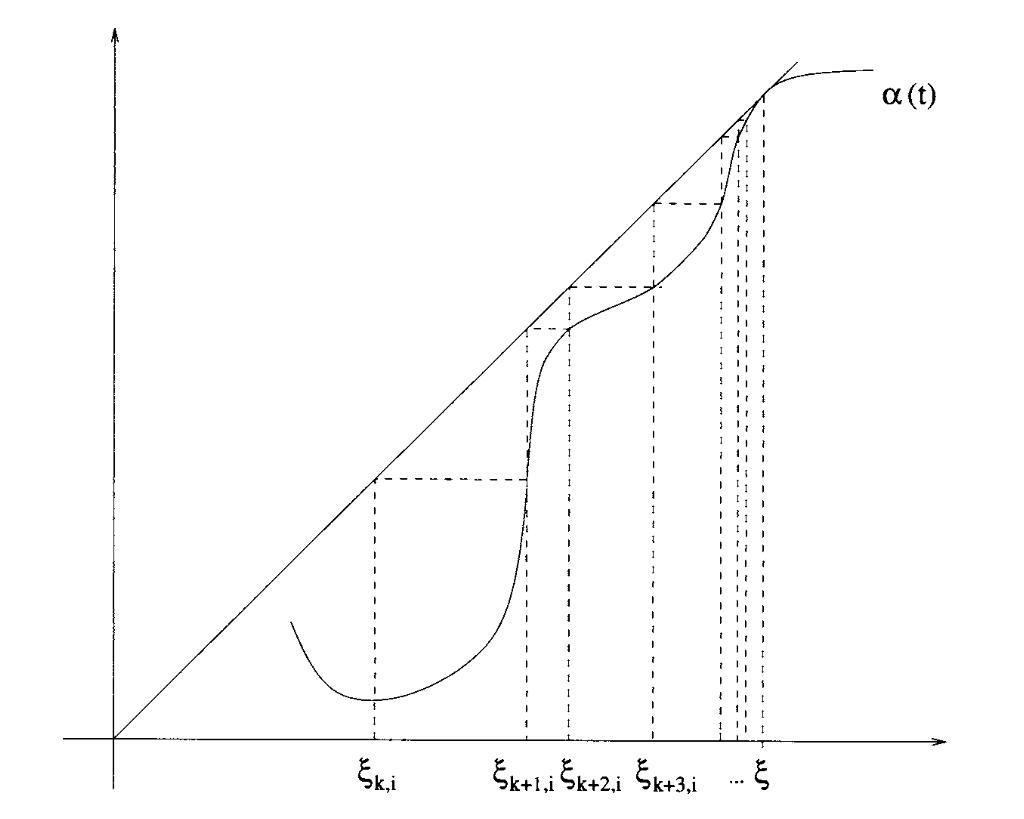
\includegraphics[width=0.7\textwidth, height=0.5\textheight]{desaparecimento_do_retardo.png}
        \end{center}
        \caption{Desaparecimento do Retardo ({\color{red} texto})}\label{fig:Desaparecimento do Retardo}
    \end{figure}


    % \begin{proof}[Demonstração ...Continuação]
    %     \[
    %         \vdots
    %     \]
    %     $\bullet$ Como $\xi$ é único ponto fixo em $[t_0, \xi]$ por hípotese, então $\lim_{n \to \infty} s_n = \xi$. Portanto, existem infinitos pontos de descontinuidade em qualquer vizinhança a esquerda de $\xi$.
    % \end{proof}
    %
    $\bullet$ Para evitar este problema, a seguinte hipótese é introduzida.

    \begin{hip}
        Existe uma constante $ \tau_0 > 0 $ tal que $ \tau(t) = t - \alpha(t) > \tau_0 $ para todo $ t \in [t_0, t_f] $.
        \label{H1:hipotese:hypothesis}
    \end{hip}




\end{frame}


% %%%%%%%%%%%%%%%%%%%%%%%%%%%%%%%%%%%%%%%%%%%%%%%%%%%%%%%%%%%%%%%%%%%%%%%%%%%%%%%%%%%%%%%%%%%%%%%%%%%%%%%
%
% \begin{frame}{Desaparecimento do Retardo}
%     
%
%     \begin{figure}
%         \begin{center}
%             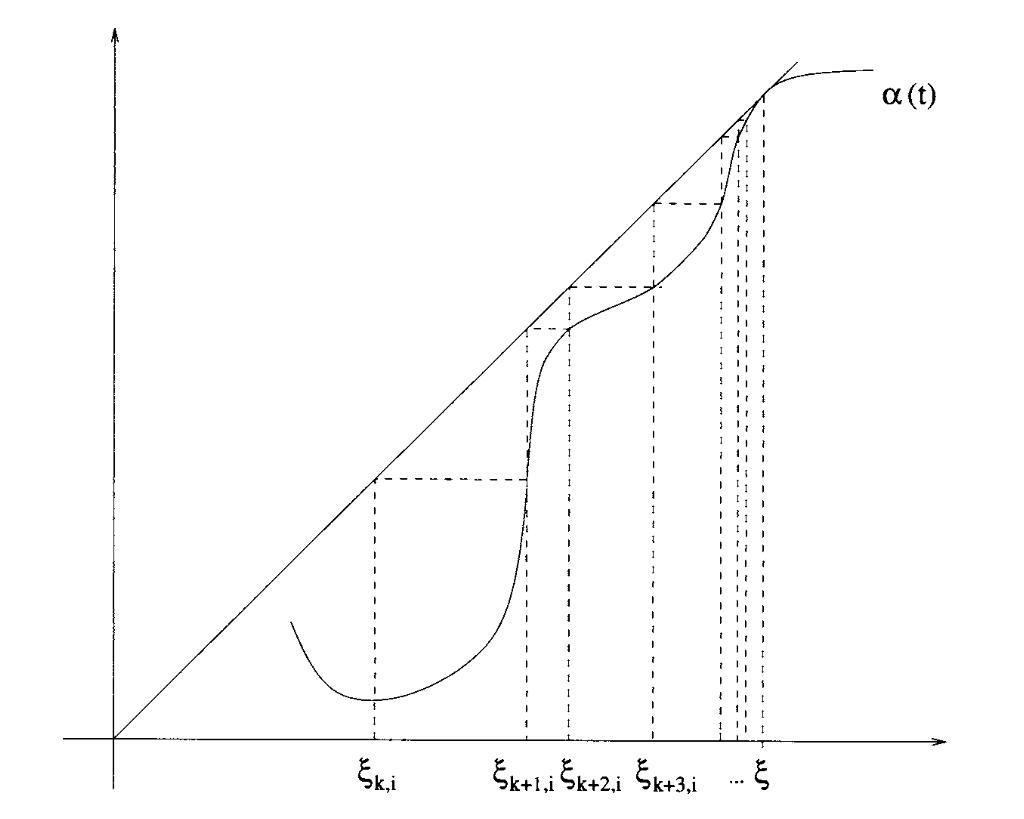
\includegraphics[width=0.9\textwidth, height=0.7\textheight]{desaparecimento_do_retardo.png}
%         \end{center}
%         \caption{Desaparecimento do Retardo (Ainda vou montar minha própria imagem)}\label{fig:Desaparecimento do Retardo}
%     \end{figure}
%         
%
% \end{frame}


%%%%%%%%%%%%%%%%%%%%%%%%%%%%%%%%%%%%%%%%%%%%%%%%%%%%%%%%%%%%%%%%%%%%%%%%%%%%%%%%%%%%%%%%%%%%%%%%%%%%%%%

\subsection{Retardos Limitados e Ilimitados}
\begin{frame}{Retardos Limitados e Ilimitados}

    \scriptsize
    $\bullet$ Caso o retardo seja limitado, a suavização da solução como visto no teorema \ref{chap2:teo:EDR_smooting}, não ocorre.

    $\bullet$ Para mostrar tanto, supoha que exista algum $M>0$ tal que \( \lim_{t \to \infty} \alpha(t) \leq M \).

    $\bullet$ Suponha que $\xi_{k, i}$ seja uma descontinuidade primária em $[M, +\infty)$, então $\alpha(t) < M < \xi_{k, j}$ para todo $t > M$, logo não existe $\xi_{k+1, i}$ que satisfaz $\alpha(\xi_{k+1, i}) = \xi_{k, j}$.

    \begin{figure}
        \begin{center}
            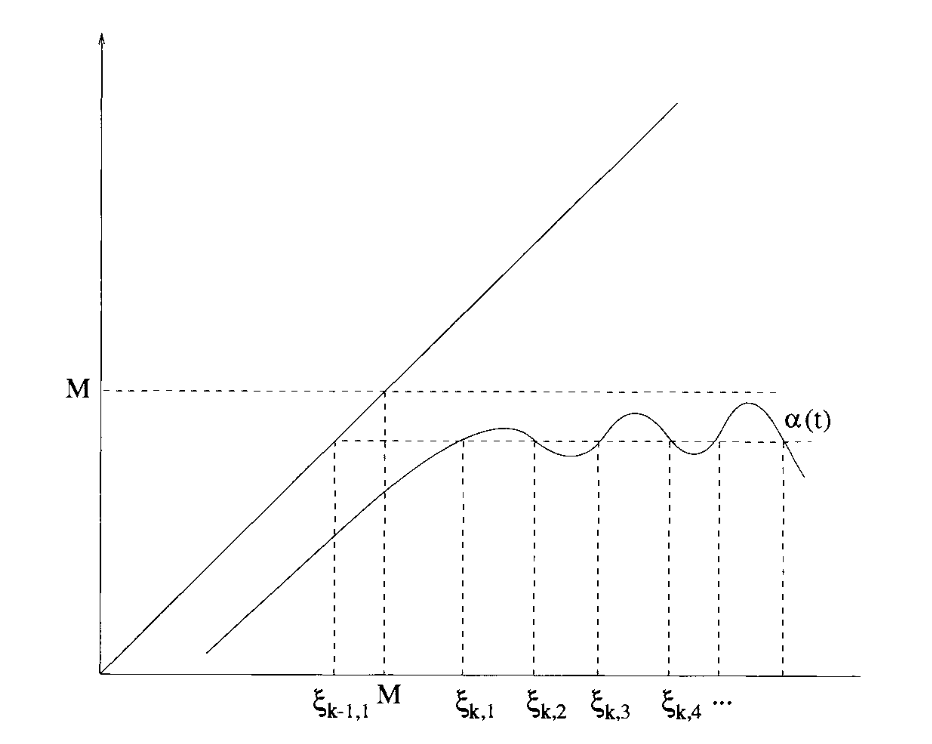
\includegraphics[width=0.7\textwidth, height=0.5\textheight]{retardo_limitado.png}
        \end{center}
        \caption{Retardo limitado ({\color{red} texto})}\label{fig:Retardo_limitado}
    \end{figure}

    % \begin{exampleblock}
    %     <1->{Retardos Limitados}
    %
    %     $\bullet$ Caso o retardo seja limitado, a suavização da solução como visto no teorema \ref{chap2:teo:EDR_smooting}, não ocorre.
    %
    %
    %     $\bullet$ Para mostrar tanto, supoha que exista algum $M>0$ tal que \( \lim_{t \to \infty} \alpha(t) \leq M \).
    %
    %     $\bullet$ Suponha que $\xi_{k, i}$ seja uma descontinuidade primária em $[M, +\infty)$, então $\alpha(t) < M < \xi_{k, j}$ para todo $t > M$, logo não existe $\xi_{k+1, i}$ que satisfaz $\alpha(\xi_{k+1, i}) = \xi_{k, j}$.
    %     
    %     $\bullet$ Segue uma ilustração deste fenômemo.
    %
    % \end{exampleblock}

\end{frame}

% %%%%%%%%%%%%%%%%%%%%%%%%%%%%%%%%%%%%%%%%%%%%%%%%%%%%%%%%%%%%%%%%%%%%%%%%%%%%%%%%%%%%%%%%%%%%%%%%%%%%%%%
%
% \begin{frame}{Retardos Limitados e Ilimitados}
%
%     \begin{figure}
%         \begin{center}
%             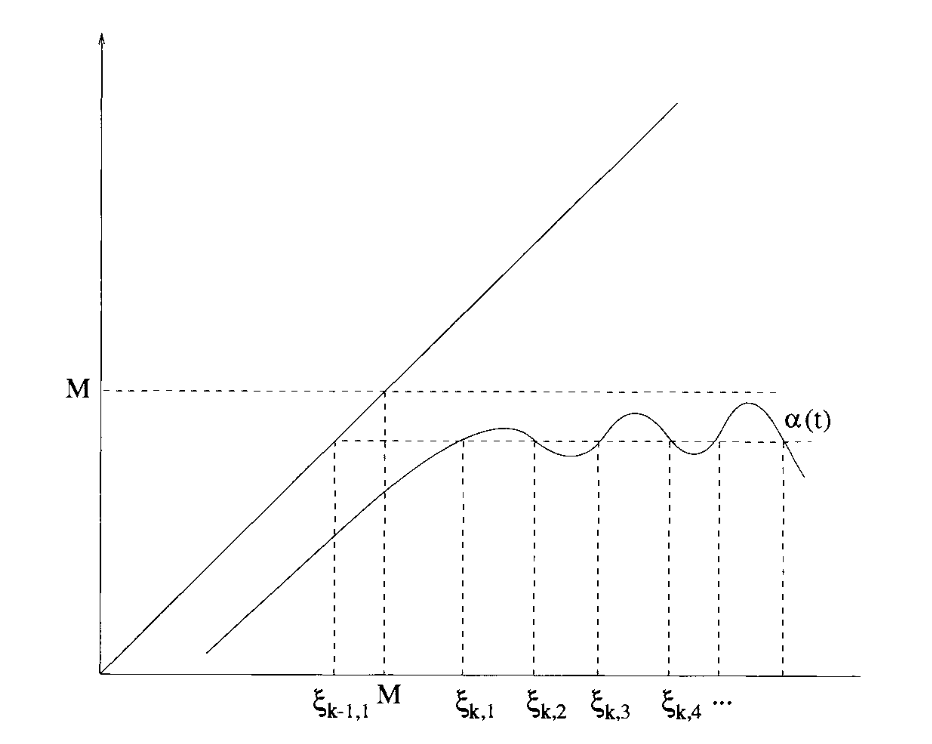
\includegraphics[width=0.9\textwidth, height=0.7\textheight]{retardo_limitado.png}
%         \end{center}
%         \caption{Retardo limitado (Ainda vou montar minha própria imagem)}\label{fig:Retardo_limitado}
%     \end{figure}
%
% \end{frame}


%%%%%%%%%%%%%%%%%%%%%%%%%%%%%%%%%%%%%%%%%%%%%%%%%%%%%%%%%%%%%%%%%%%%%%%%%%%%%%%%%%%%%%%%%%%%%%%%%%%%%%%

\begin{frame}{Retardos Limitados e Ilimitados}
    
    $\bullet$ Para garantir a suavização das soluções, a função $\alpha$ deve setisfazer as seguintes duas hipóteses.

    \begin{hip}
        \label{H2:hipotese:hypothesis}
        $\lim _{t \rightarrow+\infty} \alpha(t)=+\infty$.
    \end{hip}


    \begin{hip}
        \label{H3:hipotese:hypothesis}
        Existe uma constante \(\tau_{1}>0\) tal que \(\tau(t)=t-\alpha(t) \leq \tau_{1}\) para todo \(t \in\left[t_{0}, t_{f}\right]\).
    \end{hip}

    $\bullet$ abaixo, segue uma figura ilustrativa dessas três hipóteses em ação.

\end{frame}



%%%%%%%%%%%%%%%%%%%%%%%%%%%%%%%%%%%%%%%%%%%%%%%%%%%%%%%%%%%%%%%%%%%%%%%%%%%%%%%%%%%%%%%%%%%%%%%%%%%%%%%

\begin{frame}{Retardos Limitados e Ilimitados}

    \begin{figure}
        \begin{center}
            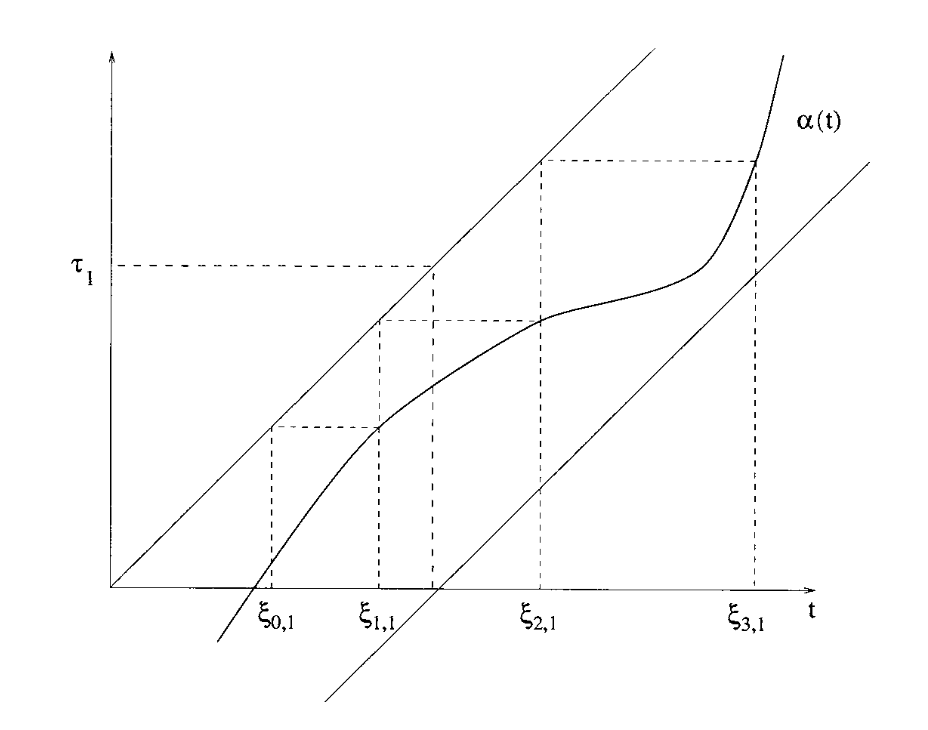
\includegraphics[width=0.9\textwidth, height=0.7\textheight]{hip123.png}
        \end{center}
        \caption{Hipóteses 1, 2 e 3 (Ainda vou montar a minha)}\label{fig:hip123}
    \end{figure}

\end{frame}


%%%%%%%%%%%%%%%%%%%%%%%%%%%%%%%%%%%%%%%%%%%%%%%%%%%%%%%%%%%%%%%%%%%%%%%%%%%%%%%%%%%%%%%%%%%%%%%%%%%%%%%




\subsection{Existência e unicidade}
\begin{frame}
     
\begin{teo}[Existência e unicidade para EDRs]
  \label{teo:local_existence:EDR}
  \small
  Considere a equação \eqref{def:eq:EDR}, ou seja,

  \[
    \left\{\begin{array}{l}
        y^{\prime}(t)=f(t, y(t), y(t-\tau(t, y(t)))), \quad t \geq t_{0}  \\
        y(t)=\phi(t), \quad t \leq t_{0}
    \end{array}\right.
  \]

  Sejam \(U \subseteq \mathbb{R}^{d}\) e \(V \subseteq \mathbb{R}^{d}\) vizinhanças de \(\phi\left(t_{0}\right)\) e \(\phi\left(t_{0}-\tau\left(t_{0}, \phi\left(t_{0}\right)\right)\right)\), respectivamente, e suponha que a função \(f(t, u, v)\) seja contínua em relação a \(t\) e Lipschitz contínua em relação a \(u\) e \(v\) em \(\left[t_{0}, t_{0}+h\right] \times U \times V\) para algum \(h>0\). Além disso, suponha que a função inicial \(\phi(t)\) seja Lipschitz contínua para \(t \leq t_{0}\) e que a função de retardo \(\tau(t, y) \geq 0\) seja contínua em relação a \(t\) e Lipschitz contínua em relação a \(y\) em \(\left[t_{0}, t_{0}+h\right] \times U\). Então o problema \ref{def:eq:EDR} tem uma única solução em \(\left[t_{0}, t_{0}+\delta\right)\) para algum \(\delta>0\) e esta solução depende continuamente dos dados iniciais.

\end{teo}
\end{frame}

%%%%%%%%%%%%%%%%%%%%%%%%%%%%%%%%%%%%%%%%%%%%%%%%%%%%%%%%%%%%%%%%%%%%%%%%%%%%%%%%%%%%%%%%%%%%%%%%%%%%%%%

\section{Métodos Numéricos Contínuos}

%WARN: REMOVED
% \subsection{Intro}
%
% \begin{frame}{Intro aqui?}
%     \begin{itemize}
%         \item[$\bullet$] Algum blalablkanla
%     \end{itemize} 
% \end{frame}

%%%%%%%%%%%%%%%%%%%%%%%%%%%%%%%%%%%%%%%%%%%%%%%%%%%%%%%%%%%%%%%%%%%%%%%%%%%%%%%%%%%%%%%%%%%%%%%%%%%%%%%


\subsection{Métodos discretos para EDOs}


\begin{frame}{Métodos discretos para EDOs}
    \small
    \phantom{aa} $\bullet$ Para $n = 0, ..., N-1$, seja $\Delta = \{ t_0, ..., t_N = t_f\}$ uma malha e $h_{n+1} = t_{n+1} - t_n$ os passos.

    \begin{defi}
        Um método numérico para resolver o PVI \eqref{def:eq:PVI} é chamado de \textbf{método de k-passos} se ele satisfaz 

        \begin{equation}
            y_{n+1} = \alpha_{n, 1} y_n + ... + \alpha_{n, k} y_{n - k + 1} + h_{n+1} \Phi( y_n, ..., y_{n-k+1}; g, \Delta_n), 
            \label{chap3:def:eq:ODE_method}
        \end{equation}

        para $n \geq k - 1$ e para $\Delta_n = \{ t_{n - k + 1}, ..., t_n, t_{n+1}\} $.

    \end{defi}

    \phantom{aa} $\bullet$ A função $\Phi$ é chamada de função incremento.

    \phantom{aa} $\bullet$ Os valores $y_0, ..., y_k$ são os valores iniciais.

    \phantom{aa} $\bullet$ A solução numérica discreta é $\{y_{n}\}_{n=0}^{N}$, onde  $y_{n} \approx y(t_{n})$.


\end{frame}

%%%%%%%%%%%%%%%%%%%%%%%%%%%%%%%%%%%%%%%%%%%%%%%%%%%%%%%%%%%%%%%%%%%%%%%%%%%%%%%%%%%%%%%%%%%%%%%%%%%%%%%

\begin{frame}{Métodos discretos para EDOs}

    \small


    \phantom{aa} $\bullet$ Caso $k = 1$, temos os chamados métodos de passo único, como o método de Euler (convergência $\mathcal{O}(h)$ para $h = \max_{n \geq 1} h_n$) 

    \[
        y_{n+1} = y_n + h_n g(t_n, y_n)
    \]

    \phantom{aa} $\bullet$ Caso $k > 1$, temos os métodos multipasso. Um exemplo de um método multipasso é o método de Adams–Bashforth de 2 passos (convergência $\mathcal{O}(h^2)$) , o qual é definido por 


    \[
        y_{n+1} = y_{n} + \frac{3}{2} h_{n+1} g(t_{n},y_{n}) - \frac{1}{2} h_{n}g(t_{n-1},y_{n-1}),
    \]

    \noindent
    e  inicializado por algum método de passo único, como o método do ponto médio (convergência $\mathcal{O}(h^2)$) descrito abaixo

    \[
        y_{n+1}=y_{n}+h_{n+1}g\left(t_{n}+{\tfrac {1}{2}}h_{n+1},y_{n}+{\tfrac{1}{2}}h_{n}g(t_{n},y_{n})\right).
    \]
\end{frame}

%%%%%%%%%%%%%%%%%%%%%%%%%%%%%%%%%%%%%%%%%%%%%%%%%%%%%%%%%%%%%%%%%%%%%%%%%%%%%%%%%%%%%%%%%%%%%%%%%%

\begin{frame}{Métodos discretos para EDOs}
    \begin{assumption}
        \label{chap3:assumption:1:Phi}
        \small
        Quanto a função incremento $\Phi$, as seguintes suposições são feitas:

        \phantom{aa} 1. $\Phi$ satisfaz uma condição Lipschitz em relação às variáveis $y$ com constante de Lipschitz $Q_g$.


        \phantom{aa} 2. Existem $h_g>0$ e $\gamma_g > 0$  tal que que $\Phi$ possui uma dependência contínua de $g$ com relação a norma do supremo no conjunto $U_n = [t_{n-k+1}, t_{n+1}] \times \R^d$, onde $h_{n - k +2 }, \dots, h_{n+1} \leq h_g (L)$, ou seja, 

        \scriptsize
            \begin{equation}
                \begin{split}
                    \| \Phi(y_n, ..., y_{n - k + 1}; \tilde{g}, \Delta_n)  &- \Phi(y_n, ..., y_{n - k + 1}; g, \Delta_n) \| \\
                                                                           &\leq \gamma_g \sup_{t, y \in U_n} \| \tilde{g}(t, y) - g(t, y) \|
                \end{split}
                \label{chap3:assumption:point_lipschitz_Phi}
            \end{equation}

        para todo $\tilde{g} \in C^0([t_0, t_f] \times \R^d, \R^d)$ . 

    \end{assumption}

\end{frame}

%%%%%%%%%%%%%%%%%%%%%%%%%%%%%%%%%%%%%%%%%%%%%%%%%%%%%%%%%%%%%%%%%%%%%%%%%%%%%%%%%%%%%%%%%%%%%%%%%%%%%%%%%%%%%% 


%%%%%%%%%%%%%%%%%%%%%%%%%%%%%%%%%%%%%%%%%%%%%%%%%%%%%%%%%%%%%%%%%%%%%%%%%%%%%%%%%%%%%%%%%%%%%%%%%%%%%%%



\subsection{Extensão Contínua}
\begin{frame}{Extensão Contínua}


    \small
    \begin{defi}[Extensão contínua]
        Uma \textbf{extensão contínua}, ou uma \textbf{interpolante} do método \eqref{chap3:def:eq:ODE_method} é uma função polinomial $\eta(t)$ definida por partes nos intervalos $[t_n, t_{n+1}]$ baseada em valores calculados pelo método definidos em $[t_{n - i_n}, t_{n+j_n + 1}]$, para $i_n, j_n \geq 0$. 

        \scriptsize
        \begin{equation}
            \begin{split}
                \eta(t_n + \theta h_{n+1}) = &\beta_{n, 1} (\theta) y_{n + j_n} + \dots + \beta_{n, j_n + i_n + 1}(\theta) y_{n - i_n} \\
                                             &+ h_{n+1} \Psi(y_{n+j_n}, \dots, y_{n-i_n}; \theta, g, \Delta _n '), \qquad 0 \leq \theta \leq 1,
                                             \label{chap3:def:eq:Interpolant_extension}
            \end{split}
        \end{equation}

        \noindent
        \normalsize
        para $\Delta _n ' = \{ t_{n - i_n} , \dots, t_{n+j_n}, t_{n +j_n + 1} \}$, onde $\eta$ satisfaz a seguinte condição de continuidade

        \scriptsize
        \begin{equation}
            \eta(t_n) = y_n \qquad  \text{ e } \qquad \eta(t_{n+1}) = y_{n+1}
            \label{chap3:def:eq:continuity_condition}
        \end{equation}

    \end{defi}

\end{frame}
 

%%%%%%%%%%%%%%%%%%%%%%%%%%%%%%%%%%%%%%%%%%%%%%%%%%%%%%%%%%%%%%%%%%%%%%%%%%%%%%%%%%%%%%%%%%%%%%%%%%%%%%%

\begin{frame}{Extensão Contínua}

    Note que

    \begin{itemize}
        \item[$\bullet$] Caso $i_n = j_n = 0$, a interpolação ocorre baseada nos valores em $[t_n, t_{n+1}]$. Tal caso é chamado de \textit{interpolação de passo único}. Caso isso não ocorra, temos uma interpolação de múltiplos passos. 
        \item[$\bullet$] Caso $j_{n} > 0$, o interpolante \eqref{chap3:def:eq:Interpolant_extension} não pode ser calculado simultâneamente com o método \eqref{chap3:def:eq:ODE_method}, devendo esperá-lo atingir o passo $t_{n + j_n + 1}$ para poder ser calculado.
    \end{itemize}


    Um método numérico discreto para EDOs acompanhado de uma extensão contínua é chamado um \textit{método numérico contínuo para EDOs}. 


\end{frame}


%%%%%%%%%%%%%%%%%%%%%%%%%%%%%%%%%%%%%%%%%%%%%%%%%%%%%%%%%%%%%%%%%%%%%%%%%%%%%%%%%%%%%%%%%%%%%%%%%%%%%%%

\begin{frame}{Extensão Contínua}

    \phantom{aa} $\bullet$ A função $\Psi$ é também chamada de função incremento. 

    \phantom{aa} $\bullet$ Para garantir a condição de continuidade de $\eta$, normalmente são consideradas as seguintes hipóteses

    \[
        \begin{gathered}
            \beta_{n, j}(0)= \begin{cases}1 & \text { para } j=1+j_{n}, \\
            0 & \text { caso contrário, }\end{cases} \\
            \Psi\left(y_{n+j_{n}}, \ldots, y_{n-i_{n}} ; 0, g, \Delta_{n}^{\prime}\right)=0
            \end{gathered}
    \]

    \[
        \begin{gathered}
            \beta_{n, j}(1)=\left\{\begin{array}{l}
                    \alpha_{n, j-j_{n}} \text { para } 1+j_{n} \leq j \leq k+j_{n} \\
                    0 \text { caso contrário }
            \end{array}\right. \\
            \Psi\left(y_{n+j_{n}}, \ldots, y_{n-i_{n}} ; 1, g, \Delta_{n}^{\prime}\right)=\Phi\left(y_{n}, \ldots, y_{n-k+1} ; g, \Delta_{n}\right).
        \end{gathered}
    \]


        \phantom{aa} $\bullet$ Para $\theta=1$, a equação \eqref{chap3:def:eq:Interpolant_extension} se reduz à \eqref{chap3:def:eq:ODE_method}. 

    \end{frame}




%%%%%%%%%%%%%%%%%%%%%%%%%%%%%%%%%%%%%%%%%%%%%%%%%%%%%%%%%%%%%%%%%%%%%%%%%%%%%%%%%%%%%%%%%%%%%%%%%%%%%%%

\begin{frame}{Extensão Contínua}
    \begin{assumption}
        \label{chap3:assumption:1:Psi}
        \small
        Quanto a função incremento $\Psi$, as seguintes suposições são feitas:

        \phantom{aa} 1. $\Psi$ satisfaz uma condição Lipschitz em relação às variáveis $y$ com constante de Lipschitz $Q_g$.


        \phantom{aa} 2. Existem $h_g'>0$ e $\gamma_g' > 0$  tal que que $\Phi$ possui uma dependência contínua de $g$ com relação a norma do supremo no conjunto $U_n ' = [t_{n-i_n}, t_{n+j_n + 1}] \times \R^d$, onde $h_{n - i_n + 1 }, \dots, h_{n+j_n + 1} \leq h_g' (L)$, ou seja, 

        \scriptsize
            \begin{equation}
                \begin{split}
                    \| \Psi(y_{n + jn}, ..., y_{n - i_n}; \tilde{g}, \Delta_n ')  &- \Psi(y_{n + jn}, ..., y_{n - i_n}; g , \Delta_n ') \| \\
           &\leq \gamma_g ' \sup_{t, y \in U_n '} \| \tilde{g}(t, y) - g(t, y) \|
                \end{split}
                \label{chap3:assumption:point_lipschitz_Psi}
            \end{equation}

            
        \small
        para todo $\tilde{g} \in C^0([t_0, t_f] \times \R^d, \R^d)$ . 

    \end{assumption}

\end{frame}


%%%%%%%%%%%%%%%%%%%%%%%%%%%%%%%%%%%%%%%%%%%%%%%%%%%%%%%%%%%%%%%%%%%%%%%%%%%%%%%%%%%%%%%%%%%%%%%%%%%%%%%
\subsection{Ordem dos métodos}


    \begin{frame}{Ordem dos métodos}

        \footnotesize
        \begin{defi}[Ordem Local de um método discreto]
            \label{chap3:def:order_of_discrete_methods}

            Um método discreto \eqref{chap3:def:eq:ODE_method}  é consistente e de ordem $p \geq 1$ é o menor inteiro tal que, para toda função $g \in C^p$ e para todos os pontos da malha tem-se que 

            \begin{equation}
                \| z_{n+1}(t_{n+1}) - \tilde{y}_{n+1} \| = \mathcal{O} (h_{n+1}^{p+1}), 
                \label{chap3:eq:order_of_discrete_methods:1}
            \end{equation}

            \noindent
            uniformemente com respeito a $y_{n}^*$ em qualquer conjunto limitado de $R^d$ e para $n = 0, ..., N-1$, onde $z_{n+1}(t)$ é solução do problema local

            \begin{equation}
                \begin{cases}
                    z_{n+1}'(t) = g(t, z_{n+1}(t)), \qquad t_n \leq t \leq t_{n+1} , \\
                    z(t_n) = y_n ^*, \qquad t \leq t_0,
                \end{cases}
                \label{chap3:eq:order_of_discrete_methods:2}
            \end{equation}


            \begin{equation}
                \begin{split}
                    \text{para} \qquad 
                    \tilde{y}_{n+1} &= \alpha_{n, 1} z_{n+1}(t_n) + \dots + \alpha_{n, k} z_{n+1}(t_{n-k+1}) \\
                                   &+ h_{n+1} \Phi(z_{n+1}(t_n), \dots, z_{n+1}(t_{n-k+1}); g, \Delta_n).
                \end{split}
                \label{chap3:eq:order_of_discrete_methods:3}
            \end{equation}

        \end{defi}

\end{frame}



%%%%%%%%%%%%%%%%%%%%%%%%%%%%%%%%%%%%%%%%%%%%%%%%%%%%%%%%%%%%%%%%%%%%%%%%%%%%%%%%%%%%%%%%%%%%%%%%%%%%%%%

\begin{frame}{Ordem dos métodos}


    \small
    \begin{defi}[Ordem Local do interpolante]
        \label{chap3:def:interpolant_extension_order}

        Um interpolante \eqref{chap3:def:eq:Interpolant_extension} é consistente e de ordem $q \geq 1$ se


        \begin{equation}
            \max_{t_n \leq t \leq t_{n+1}}\| z_{n+1}(t) - \tilde{ \eta }_{n+1}(t) \| = \mathcal{O} (h_{n+1}^{q+1}), 
            \label{chap3:eq:Interpolant_extension_order}
        \end{equation}

        para 

        \begin{equation}
            \begin{split}
                \tilde{\eta}(t_{n} + \theta h_{n+1}) &= \beta_{n, 1}(\theta) z_{n+1}(t_{n+j_n}) + \dots + \beta_{n, j_n + i_n + 1}(\theta) z_{n+1}(t_{n-i_n}) \\
                                                     &+ h_{n+1} \Psi(z_{n+1}(t_{n+ j_n}), \dots, z_{n+1}(t_{n-i_n}); \theta,  g, \Delta_n ')
            \end{split}
            \label{chap3:def:interpolant_extension_order:eq:1}
        \end{equation}

    \end{defi}

\end{frame}



%%%%%%%%%%%%%%%%%%%%%%%%%%%%%%%%%%%%%%%%%%%%%%%%%%%%%%%%%%%%%%%%%%%%%%%%%%%%%%%%%

\begin{frame}{Ordem dos métodos}

    \small

    \phantom{aa} $\bullet$ Seja $h = \max_{1 \leq n \leq N} h_n$.


    \begin{defi}[Ordem Global de um Método Discreto]
        
        Um método discreto \eqref{chap3:def:eq:ODE_method} tem ordem global $p$, se 

        \begin{equation}
            \max_{1 \leq n \leq N} \| y(t_n) - y_n \| = \mathcal{O}(h^p),
        \end{equation}
    \end{defi}


    \begin{defi}[Ordem Global de um Interpolante]
        
        Um interpolante \eqref{chap3:def:eq:Interpolant_extension} tem ordem global $p$, se 

        \begin{equation}
            \max_{t_0 - r \leq t \leq t_f} \| y(t) - \eta(t) \| = \mathcal{O}(h^{p}).
        \end{equation}
    \end{defi}

\end{frame}
%%%%%%%%%%%%%%%%%%%%%%%%%%%%%%%%%%%%%%%%%%%%%%%%%%%%%%%%%%%%%%%%%%%%%%%%%%%%%%%%%

\subsection{Teorema de convergência}

\begin{frame}{Preliminares para o teorema de convergência}
    \begin{defi}[Norma induzida de matrizes]
        \label{apendices:def:induced_matrix_norm}
        Seja $K$ o corpo dos reais ou dos complexos e sejam $\|\cdot\|_\alpha$ e $\|\cdot\|_\beta$ normas em $K^n$ e $K^m$, respectivamente.
        A norma $\| \cdot \|_{\alpha, \beta}$ em $K^{m \times n}$ é chamada de \textit{norma induzida} se 

        \[ \| A \|_{\alpha, \beta} = \sup\left\{\frac{\|Ax\|_\beta}{\|x\|_\alpha} : x\in K^n \backslash \left\{0\right\} \right\}. \]


        Normalmente, a notação a acima é reduzida simplesmente a 

        \[ \| A \|_{\alpha, \beta} = \sup_{\|x\|_\alpha = 1} \|Ax\|_\beta.\]

    \end{defi}


\end{frame}

%%%%%%%%%%%%%%%%%%%%%%%%%%%%%%%%%%%%%%%%%%%%%%%%%%%%%%%%%%%%%%%%%%%%%%%%%%%%%%%%

\begin{frame}{Preliminares para o teorema de convergência}

    \small
    \begin{defi}[Produto de Kronecker]
        \label{apendices:def:kronecker_product}
        Sejam $A$ e $B$ duas matrizes quaisquer nos espaços vetorias $K^{m, n}, m,n \geq 0$ e $B \in K^{p, q}, r,s \geq 0$ 
        para $K = \R$ (ou $\C$). O \textit{produto Kronecker} entre $A$ e $B$ é dado pela função
        $\otimes: K^{m, n} \times K^{p, q} \to (K^{pm \times qn})$ definida notação por blocos

        \[
            A \otimes B = 
            \begin{bmatrix}
                a_{1,1} B & a_{1,2} B & \dots & a_{1, n} B \\
                a_{2,1} B & a_{2,2} B & \dots & a_{2, n} B \\
                \vdots & \vdots & \ddots & \vdots \\
                a_{m,1} B & a_{m,2} B & \dots & a_{m, n} B \\
            \end{bmatrix},
        \]


    \end{defi}

     
\end{frame}


%%%%%%%%%%%%%%%%%%%%%%%%%%%%%%%%%%%%%%%%%%%%%%%%%%%%%%%%%%%%%%%%%%%%%%%%%%%%%%%%%%%%%%%%%%%%%%%%%%%%%%%

\begin{frame}%{Teorema: Convergência dos Métodos para EDOs}
    \begin{teo}[Convergência dos Métodos para EDOs]
        \label{chap3:teo:continuous_ODE}
        \scriptsize
        Considere o método \eqref{chap3:def:eq:ODE_method} de ordem $p \geq 1$ e, para cada $n$, seja

        \tiny
        \[
            C_n = 
            \begin{bmatrix}
                \alpha_{n, 1} & \alpha_{n, 2} & \cdots  & \alpha_{n, k - 1} & \alpha_{n, k} \\
                1 & 0 & \cdots & 0 & 0 \\
                0 & 1 & \cdots & 0 & 0 \\
                \vdots & \vdots & \ddots & \vdots & \vdots \\
                0 & 0 & \cdots & 1 & 0 \\
            \end{bmatrix}
        \]


        \scriptsize
        Caso 

        \phantom{aa} $\bullet$ Existe uma norma $\| \cdot \|_* $ em $\R^k$, independente de $n$ e da malha $\Delta$, tal que, para a norma induzida da matriz, a seguinte condição de estabilidade é satisfeita.

        \begin{equation}
            \| C_n \|_* \leq 1.
            \label{chap3:teo:ODE_methods_convergence:eq:stability_condition}
        \end{equation}

        \phantom{aa} $\bullet$ A função $g$ de \eqref{def:eq:PVI} é $C^p$ contínua;

        \phantom{aa} $\bullet$ Os valores iniciais $y_0, \cdots, y_{k-1}$ aproxima a solução exata com ordem $p$.

        Então, o método discreto \eqref{chap3:def:eq:ODE_method} é convergente e de ordem global $p$ em $[t_0, t_f]$, já a extensão contínua \eqref{chap3:def:eq:Interpolant_extension} é convergente sua ordem global é $q' = \min\{p, q+1\}$.
    \end{teo}


\end{frame}


%%%%%%%%%%%%%%%%%%%%%%%%%%%%%%%%%%%%%%%%%%%%%%%%%%%%%%%%%%%%%%%%%%%%%%%%%%%%%%%%%%%%%%%%%%%%%%%%%%%%%%%

\begin{frame}{Teorema: Demonstração}
    \small

    \phantom{aa} $\bullet$ Como o método discreto \eqref{chap3:def:eq:ODE_method} tem ordem $p$, então 

    
    \begin{equation}
      \begin{aligned}
        y\left(t_{n+1}\right)= & \alpha_{n, 1} y\left(t_{n}\right)+\cdots+\alpha_{n, k} y\left(t_{n-k+1}\right) \\
        & +h_{n+1} \Phi\left(y\left(t_{n}\right), \ldots, y\left(t_{n-k+1}\right) ; g, \Delta_{n}\right)+\epsilon_{n+1} 
      \end{aligned}
      \label{chap3:teo:ODE_methods_convergence:eq:1}
    \end{equation}

    
    com

    \begin{equation}
      \left\|\epsilon_{n+1}\right\| \leq c h_{n+1}^{p+1}, 
      \label{chap3:teo:ODE_methods_convergence:eq:6}
    \end{equation}


    \noindent
    para alguma constante \(c>0\) e para todo \(n=k-1, \ldots, N-1\). 

   \phantom{aa} $\bullet$ Para os mesmos $n$, introduziremos a seguinte notação por blocos

    \begin{equation*}
        \begin{split}
            &\mathbf{y}_{n}=\left[y_{n}, y_{n-1}, \ldots, y_{n-k+1}\right]^{T}, \\
            &\mathbf{y}(t_{n})=[y(t_{n}), y(t_{n-1}), \ldots, y(t_{n-k+1})]^{T}.
        \end{split}
    \end{equation*}

\end{frame}



%%%%%%%%%%%%%%%%%%%%%%%%%%%%%%%%%%%%%%%%%%%%%%%%%%%%%%%%%%%%%%%%%%%%%%%%%%%%%%%%%%%%%%%%%%%%%%%%%%%%%%%

\begin{frame}{Teorema: Demonstração}
    
    \phantom{aa} $\bullet$ Note que $\mathbf{y}_n, \mathbf{y}(t_n) \in \R^{kd}$. Agora, defina \(\mathcal{C}_{n}\) por

    \[
      \mathcal{C}_{n}=C_{n} \otimes I_{d}.
    \]

    \noindent
    \phantom{aa} $\bullet$  Então que $\mathcal{C}_{n}$ é uma matriz $(dk)\times(dk)$ dada por

    \[
      \mathcal{C}_{n}  = 
      \begin{bmatrix}
        \alpha_{n,1} I_d & \alpha_{n,2} I_d & \dots & \alpha_{n, k-1} I_d & \alpha_{n, k} I_d \\
        I_d & 0 & \dots & 0 & 0 \\
        0 & I_d & \dots & 0 & 0 \\
        \vdots & \vdots & \ddots & \vdots & \vdots \\
        0 & 0 & \dots & I_d & 0 \\
      \end{bmatrix}.
    \]

\end{frame}


%%%%%%%%%%%%%%%%%%%%%%%%%%%%%%%%%%%%%%%%%%%%%%%%%%%%%%%%%%%%%%%%%%%%%%%%%%%%%%%%%%%%%%%%%%%%%%%%%%%%%%%

\begin{frame}{Teorema: Demonstração}
    
    \phantom{aa} $\bullet$ Devemos mostrar que $\mathcal{C}_n$ herda a propriedade de estabilidade \eqref{chap3:teo:ODE_methods_convergence:eq:stability_condition}. Para tanto, considere $\mathbf{x} \in \R^{kd}$ qualquer. Pela notação de blocos, podemos representar $\mathbf{x}$ por $k$ blocos de vetores $x_1, \dots, x_k$  em $\R^d$, ou seja,

  \[
    \mathbf{x} = 
    \begin{bmatrix}
      x_1 \\
      x_2 \\
      \vdots \\
      x_k
    \end{bmatrix}
    =
    \begin{bmatrix}
      (x_{1}^{(1)} ,& x_{1}^{(2)} ,& \dots ,&x_{1}^{(d)})^T \\
      (x_{2}^{(1)} ,& x_{2}^{(2)} ,& \dots ,&x_{2}^{(d)})^T \\
      \vdots & \vdots  &\phantom{\dots} &\vdots \\
      (x_{k}^{(1)} ,& x_{k}^{(2)} ,& \dots ,&x_{k}^{(d)})^T \\
    \end{bmatrix}.
  \]
\end{frame}


%%%%%%%%%%%%%%%%%%%%%%%%%%%%%%%%%%%%%%%%%%%%%%%%%%%%%%%%%%%%%%%%%%%%%%%%%%%%%%%%%%%%%%%%%%%%%%%%%%%%%%%

\begin{frame}{Teorema: Demonstração}


    \phantom{aa} $\bullet$ A a norma que utilizaremos para trabalhar em $\R^{kd}$ será a norma do máximo definida como
    
    \begin{equation}
      \vertiii{\mathbf{x}} = \max_{1 \leq i \leq d} \|x^{(i)}\|_* ,
      \label{chap3:teo:ODE_methods_convergence:eq:norm}
    \end{equation}
 
    \noindent
    onde cada \(x^{(i)}\) é o vetor $x^{(i)} = (x_1 ^{(i)}, \dots, x_k ^{(i)})^T \in \R^k$.


    \phantom{aa} $\bullet$ Para  $\mathcal{C}_n$ satisfaz \eqref{chap3:teo:ODE_methods_convergence:eq:stability_condition}, ou seja,  $\vertiii{\mathcal{C}_n} \leq 1$, basta mostrar que $\vertiii{ \mathcal{C}_n \mathbf{x}} \leq \vertiii{\mathbf{x}}$. Para tanto, teremos

    % \phantom{aa} $\bullet$ Para provar que $\mathcal{C}_n$ satisfaz \eqref{chap3:teo:ODE_methods_convergence:eq:stability_condition}, pela definição da norma induzida \ref{apendices:def:induced_matrix_norm}, basta mostrar que $\vertiii{ \mathcal{C}_n \mathbf{x}} \leq \vertiii{\mathbf{x}}$ para todo $\mathbf{x}$. Teremos, então, que


    \scriptsize
    \[
      \mathcal{C}_{n} \mathbf{x}  = 
      \begin{bmatrix}
        \alpha_{n,1} I_d & \alpha_{n,2} I_d & \dots & \alpha_{n, k-1} I_d & \alpha_{n, k} I_d \\
        I_d & 0 & \dots & 0 & 0 \\
        0 & I_d & \dots & 0 & 0 \\
        \vdots & \vdots & \ddots & \vdots & \vdots \\
        0 & 0 & \dots & I_d & 0 \\
      \end{bmatrix}
      \begin{bmatrix}
        x_1 \\
        x_2 \\
        x_3 \\
        \vdots \\
        x_k
      \end{bmatrix} =
      \begin{bmatrix}
        \alpha_{n,1}x_1 + \dots + \alpha_{n, k} x_k \\
        x_1 \\
        x_2 \\
        \vdots \\
        x_{k-1}
      \end{bmatrix}
    \]

\end{frame}


%%%%%%%%%%%%%%%%%%%%%%%%%%%%%%%%%%%%%%%%%%%%%%%%%%%%%%%%%%%%%%%%%%%%%%%%%%%%%%%%%%%%%%%%%%%%%%%%%%%%%%%

\begin{frame}{Teorema: Continuação}
    \small

    \phantom{aa} $\bullet$ Observe que, para todo $1 \leq j \leq d$, o vetor coluna do lado direito da igualdade acima é dado por

    \[
        \begin{bmatrix}
          \alpha_{n,1}x_1 ^{(j)} + \dots + \alpha_{n, k} x_k^{(j)} \\
          x_1^{(j)} \\
          x_2 ^{(j)}\\
          \vdots \\
          x_{k-1}^{(j)}
        \end{bmatrix}
        = 
          C_n x^{(j)}.
    \]

    \phantom{aa} $\bullet$ Pela propriedade da estabilidade \eqref{chap3:teo:ODE_methods_convergence:eq:stability_condition} sobre $C_n$, temos que $\| C_n x^{(j)} \|_* \leq \| x^{(j)} \|_*$. 

    \phantom{aa} $\bullet$ Finalmente, como $\vertiii{ \mathcal{C}_{n} \mathbf{x}} \leq \|x^{(j)}\|_*$ para todo $1 \leq j \leq d$, então $\vertiii{ \mathcal{C}_{n} \mathbf{x}} \leq \vertiii{\mathbf{x}}$ e $\mathcal{C}_n$ satisfaz a propriedade.
\end{frame}

%%%%%%%%%%%%%%%%%%%%%%%%%%%%%%%%%%%%%%%%%%%%%%%%%%%%%%%%%%%%%%%%%%%%%%%%%%%%%%%%%%%%%%%%%%%%%%%%%%%%%%%

\begin{frame}{Teorema: Continuação}

    \small

    \phantom{aa} $\bullet$ Pela notação de blocos, temos que $y(t_n) - y_n$ é equivalente a 

    \begin{equation}
      \mathbf{y}\left(t_{n+1}\right)-\mathbf{y}_{n+1}=\mathcal{C}_{n}\left(\mathbf{y}\left(t_{n}\right)-\mathbf{y}_{n}\right)+h_{n+1} \Gamma_{n}+E_{n+1}, \quad n=k-1, \ldots, N-1 
      \label{chap3:teo:ODE_methods_convergence:eq:5}, 
    \end{equation}
  
    \noindent
    onde

    \begin{align*}
      &\Gamma_{n}=\left(\Phi\left(\mathbf{y}\left(t_{n}\right) ; g, \Delta_{n}\right)-\Phi\left(\mathbf{y}_{n} ; g, \Delta_{n}\right), 0, \ldots, 0\right)^{T}, \\
      &E_{n+1}=\left(\epsilon_{n+1}, 0, \ldots, 0\right)^{T},
    \end{align*}

    \noindent
    sendo 0 o vetor nulo em \(\mathbb{R}^{d}\). 

    \phantom{aa} $\bullet$ Aplicando a norma $\vertiii{\cdot}$ em ambos os lados de \eqref{chap3:teo:ODE_methods_convergence:eq:5} e utilizando da propriedade de estabilidade de $\mathcal{C}_n$, obtemos

\end{frame}


%%%%%%%%%%%%%%%%%%%%%%%%%%%%%%%%%%%%%%%%%%%%%%%%%%%%%%%%%%%%%%%%%%%%%%%%%%%%%%%%%%%%%%%%%%%%%%%%%%%%%%%

\begin{frame}{Teorema: Continuação}

    \small

    \[
      \vertiii{\mathbf{y}(t_{n+1})-\mathbf{y}_{n+1}} \leq \vertiii{\mathbf{y}(t_{n})-\mathbf{y}_{n}}+h_{n+1} \vertiii{\Gamma _ { n }} + \vertiii{E_{n+1} },
    \]

    \noindent
    para todo \(n=k-1, \ldots, N-1\).

    \phantom{aa} $\bullet$ Utilizando da propriedade da equivalência das normas em espaços de dimensão finita, obtemos 

    \[
      \begin{aligned}
        \vertiii{E_{n+1}} &= \max_{1 \leq i \leq d} \| (e_{n+1}^{(i)}, 0, \dots, 0) \|_* \leq 
        \max_{1 \leq i \leq d} ( k_1 \| (e_{n+1}^{(i)}, 0, \dots, 0) \|_\infty ) \\
                          &\leq k_1 \max_{1 \leq i \leq d} |e_{n+1}^{(i)}| 
        \leq k_1 \|e_{n+1}^{(i)}\|_\infty  \\
                          &\leq k_1 k_2 \|e_{n+1}\| \leq k_1 k_2 c h_{n+1}^{p+1} \leq k_1 k_2 c h_{n+1} h^{p},
      \end{aligned}
    \]

    \noindent
    para algum $k_1, k_2 > 0$ e para $h = \max_{1 \leq n \leq N} h_n$.
\end{frame}

%%%%%%%%%%%%%%%%%%%%%%%%%%%%%%%%%%%%%%%%%%%%%%%%%%%%%%%%%%%%%%%%%%%%%%%%%%%%%%%%%%%%%%%%%%%%%%%%%%%%%%%

\begin{frame}{Teorema: Continuação}
    \phantom{aa} $\bullet$ Quanto ao restante da normas, pela continuidade Lipschitz da função incremento \(\Phi\) em relação aos argumentos \(y\) na norma \(\|\cdot\|\) em \(\mathbb{R}^{d}\) e, novamente, pela propriedade de equivalência das normas, junto com \eqref{chap3:teo:ODE_methods_convergence:eq:6}, existe uma constante \(Q>0\) tal que, para $c' = k_1 k_2$ e para todo $n = k - 1, \dots, N -1$, temos

    \[
      \vertiii{\mathbf{y}(t_{n+1})-\mathbf{y}_{n+1}} \leq (1+h_{n+1} Q) \vertiii{\mathbf{y}(t_{n})-\mathbf{y}_{n}} 
      +c^{\prime} h_{n+1} h^{p}.
    \]

    \phantom{aa} $\bullet$ Observe que $1 + h_j Q \leq e^{h_j Q}$ para todo $j$, assim, continuando a relação de recorrência, obtemos

\end{frame}


%%%%%%%%%%%%%%%%%%%%%%%%%%%%%%%%%%%%%%%%%%%%%%%%%%%%%%%%%%%%%%%%%%%%%%%%%%%%%%%%%%%%%%%%%%%%%%%%%%%%%%%

\begin{frame}{Teorema: Continuação}
    \begin{align*}
        \vertiii{\mathbf{y}(t_{n+1})-\mathbf{y}_{n+1}} \leq & \overbrace{^{h_{n+1}Q} \dots e^{h_{k}Q} \vertiii{\mathbf{y}(t_{k-1})-\mathbf{y}_{k-1}}}^{(\star)} \\
                                                            &+ \underbrace{c' h^p (h_{n+1} + e^{h_{n+1}Q}h_n + \dots + e^{(h_{n+1} \dots h_{k+1})Q}h_k)}_{(\star \star)}.
    \end{align*}

    \phantom{aa} $\bullet$ Quanto a $(\star)$, observe que, como $h_k + \dots h_{n+1} \leq t_f - t_0$, então

    \begin{align*}
      e^{h_{n+1}Q} \dots e^{h_{k}Q} \vertiii{\mathbf{y}(t_{k-1})-\mathbf{y}_{k-1}} &= e^{Q(h_{n+1} + \dots + h_k)} \vertiii{\mathbf{y}(t_{k-1})-\mathbf{y}_{k-1}} \\
                                                                                   &\leq e^{Q(t_f - t_0)} \vertiii{\mathbf{y}(t_{k-1})-\mathbf{y}_{k-1}},
    \end{align*}
\end{frame}


%%%%%%%%%%%%%%%%%%%%%%%%%%%%%%%%%%%%%%%%%%%%%%%%%%%%%%%%%%%%%%%%%%%%%%%%%%%%%%%%%%%%%%%%%%%%%%%%%%%%%%%

\begin{frame}{Teorema: Continuação}
    \noindent
    \phantom{aa} $\bullet$ Quando a $(\star \star)$, temos que

    

    \[
        \begin{split}
            h_{n+1} + e^{h_{n+1}Q}h_n &+ \dots + e^{(h_{n+1} \dots h_{k+1})Q}h_k = 
            \sum_{r = k}^{n+1}e^{\left( Q \sum_{s = r + 1}^{n+1}h_s \right)} h_r \\
            &\leq \int_{t_0}^{t_f} e^{Q(t_f - t)} \, dt = \frac{e^{Q(t_f - t_0)} - 1}{Q}
        \end{split}
    \]

    \phantom{aa} $\bullet$ Por fim, concluímos o resultado da convergência discreta com a relação final

    \[
      \vertiii{  \mathbf{y}(t_{n+1})-\mathbf{y}_{n+1} } \leq e^{Q(t_{f}-t_{0})} \vertiii{ \mathbf{y}(t_{k-1})-\mathbf{y}_{k-1} }
      +\frac{e^{Q(t_{f}-t_{0})}-1}{Q} c' h^{p}
    \]
\end{frame}



%%%%%%%%%%%%%%%%%%%%%%%%%%%%%%%%%%%%%%%%%%%%%%%%%%%%%%%%%%%%%%%%%%%%%%%%%%%%%%%%%%%%%%%%%%%%%%%%%%%%%%%

\begin{frame}{Teorema: Continuação}

    \phantom{aa} $\bullet$ Quanto ao resultado de ordem uniforme global, suponha novamente \(y_{n}^{*}=y\left(t_{n}\right)\) em \eqref{chap3:eq:order_of_discrete_methods:2} , de modo que \eqref{chap3:def:interpolant_extension_order:eq:1} fornece 

    \begin{equation}
      \begin{aligned}
        y(t_{n}+\theta h_{n+1})= & \beta_{n, 1}(\theta) y(t_{n+j_{n}})+\ldots+\beta_{n, j_{n}+i_{n}+1}(\theta) y(t_{n-i_{n}}) \\
        & +h_{n+1} \Psi(y(t_{n+j_{n}}), \ldots, y(t_{n-i_{n}}) ; \theta, g, \Delta_{n}^{\prime})+\epsilon_{n+1}(\theta) 
      \end{aligned}
      \label{chap3:teo:ODE_methods_convergence:eq:7}
    \end{equation}

    \noindent
    \phantom{aa} $\bullet$ Sendo $\max _{0 \leq \theta \leq 1}\|\epsilon_{n+1}(\theta)\| \leq \mathcal{O}(h_{n+1}^{q+1})$ para todo $n = 1, \dots, N-1$, de acordo coma definição \eqref{chap3:eq:Interpolant_extension_order}. Logo

    \begin{equation}
      \max _{0 \leq n \leq N-1} \max _{0 \leq \theta \leq 1}\left\|\epsilon_{n+1}(\theta)\right\|=O\left(h^{q+1}\right)
      \label{chap3:teo:ODE_methods_convergence:eq:8}
    \end{equation}


\end{frame}



%%%%%%%%%%%%%%%%%%%%%%%%%%%%%%%%%%%%%%%%%%%%%%%%%%%%%%%%%%%%%%%%%%%%%%%%%%%%%%%%%%%%%%%%%%%%%%%%%%%%%%%

\begin{frame}{Teorema: Continuação}

    \phantom{aa} $\bullet$  Subtraindo \eqref{chap3:def:eq:Interpolant_extension} de \eqref{chap3:teo:ODE_methods_convergence:eq:7}, utilizando da estimativa já demonstrada \eqref{chap3:eq:Interpolant_extension_order} e a da estimativa \eqref{chap3:teo:ODE_methods_convergence:eq:8}, junto com a suposição de que os termos \(\beta_{n, i}(\theta)\) são limitados uniformemente e de que a função incremento \(\Psi\) é Lipschitz continua em relação aos argumentos \(y\), obtemos
    \[
      \max _{0 \leq n \leq N-1} \max _{0 \leq \theta \leq 1}\left\|y\left(t_{n}+\theta h_{n+1}\right)-\eta\left(t_{n}+\theta h_{n+1}\right)\right\| \leq O\left(h^{p}\right)+O\left(h^{q+1}\right)
    \]

    \noindent 
     Concluindo o teorema.
\end{frame}


%%%%%%%%%%%%%%%%%%%%%%%%%%%%%%%%%%%%%%%%%%%%%%%%%%%%%%%%%%%%%%%%%%%%%%%%%%%%%%%%%%%%%%%%%%%%%%%%%%%%%%%

\subsection{Métodos Contínuos para EDRs}

\begin{frame}{Métodos Contínuos para EDRs}

    Utilizando do método dos passos, generalizaremos os métodos contínuos para EDOs para EDRs

    \phantom{aa} $\bullet$ Considere o PI de EDRs \eqref{def:eq:EDR}, ou seja,

    \begin{equation}
        \begin{cases}
            y'(t) = f(t, y(t), y(t - \tau(t, y(t)))), \qquad t_0 \leq t \leq t_f , \\
            y(t) = \phi(t), \qquad t_0 - p \leq t \leq t_0,
        \end{cases}
        \label{chap3:def:EDR}
    \end{equation}


    \phantom{aa} $\bullet$ Considere uma malha \(\Delta=\left\{t_{0}, t_{1}, \ldots, t_{n}, \ldots\right., \left.t_{N}=t_{f}\right\}\) 


    \phantom{aa} $\bullet$ Durante o $n-$ésimo passo, uma aproximação \( y_{n} \) é obtida em \( t_{n} \), o próximo passo \((n+1)\) consiste em resolver, pelo método \ref{chap3:def:eq:ODE_method}, a equação



\end{frame}


%%%%%%%%%%%%%%%%%%%%%%%%%%%%%%%%%%%%%%%%%%%%%%%%%%%%%%%%%%%%%%%%%%%%%%%%%%%%%%%%%%%%%%%%%%%%%%%%%%%%%%%

\begin{frame}{Métodos Contínuos para EDRs}

    \footnotesize

    \begin{equation}
        \left\{\begin{array}{l}
                w_{n+1}^{\prime}(t)=f(t, w_{n+1}(t), x(t-\tau(t, w_{n+1}(t)))), \quad t_{n} \leq t \leq t_{n+1} \\
                w_{n+1}(t_{n})=y_{n}
        \end{array}\right.
        \label{chap3:sec:2:eq:1}
    \end{equation}

    onde

    $$
    x(s)=\left\{\begin{array}{l}
            \phi(s) \quad \text { para } s \leq t_{0} \\
            \eta(s) \quad \text { para } t_{0} \leq s \leq t_{n} \\
            w_{n+1}(s) \quad \text { para } t_{n} \leq s \leq t_{n+1}
    \end{array}\right.
    $$

    e \(\eta(t)\) é o interpolante dado por \ref{chap3:def:eq:Interpolant_extension}. 

    \phantom{aa} $\bullet$ Se \( s=t-\tau\left(t, w_{n+1}(t)\right) \leq t_{n}$ para todo $t \in\left[t_{n}, t_{n+1}\right]\), então \eqref{chap3:sec:2:eq:1} se reduz a uma EDO.
    
    \phantom{aa} $\bullet$ Caso contrário, $\eta$ ainda aproxima $x(s)$ mas de forma implicita.
\end{frame}


%%%%%%%%%%%%%%%%%%%%%%%%%%%%%%%%%%%%%%%%%%%%%%%%%%%%%%%%%%%%%%%%%%%%%%%%%%%%%%%%%%%%%%%%%%%%%%%%%%%%%%%

\begin{frame}{Métodos Contínuos para EDRs}

    Se \( s=t-\tau\left(t, w_{n+1}(t)\right) \leq t_{n}$ para todo $t \in\left[t_{n}, t_{n+1}\right]\), então, neste intervalo

    \begin{itemize}
        \item[$\bullet$] \( x(s) \) é igual ao interpolante \(\eta(s)\). 

        \item[$\bullet$]  O problema local \eqref{chap3:sec:2:eq:1} se reduz a uma EDO. 

        \item[$\bullet$] A solução local \( w_{n+1}(t) \) é então aproximada pelo método discreto \eqref{chap3:def:eq:ODE_method} e a aproximação de \( w_{n+1}\left(t_{n+1}\right) \) é definida como \( y_{n+1} \).

    \end{itemize}

    Se \( s=t-\tau\left(t, w_{n+1}(t)\right)>t_{n} \) para algum \( t \in\left[t_{n}, t_{n+1}\right] \), então

    \begin{itemize}
        \item[$\bullet$] O valor \( x(s) \) é igual a \( w_{n+1}(s) \) e é desconhecido. Portanto, \eqref{chap3:def:EDR} não pode mais ser visto como uma EDO. 

        \item[$\bullet$] No entanto, \( x(s) \) ainda é aproximado pelo interpolante \( \eta(t) \) no intervalo subjacente \( \left[t_{n}, t_{n+1}\right] \), implicitamente definido por \eqref{chap3:def:eq:Interpolant_extension} com \( j_{n}=0\) , ou seja, por
    \end{itemize}





\end{frame}


%%%%%%%%%%%%%%%%%%%%%%%%%%%%%%%%%%%%%%%%%%%%%%%%%%%%%%%%%%%%%%%%%%%%%%%%%%%%%%%%%%%%%%%%%%%%%%%%%%%%%%%

\begin{frame}{Métodos Contínuos para EDRs}
    \begin{equation}
        \begin{split}
            \eta(t_n + \theta h_{n+1}) = &\beta_{n, 1} (\theta) y_{n} + \dots + \beta_{n, j_n + i_n + 1}(\theta) y_{n - i_n} \\
                                         &+ h_{n+1} \Psi(y_{n+j_n}, \dots, y_{n-i_n}; \theta, g_\eta, \Delta _n '), \qquad 0 \leq \theta \leq 1,
                                         \label{chap3:sec:2:def:eq:Interpolant_extension}
        \end{split}
    \end{equation}


    onde

    $$
    g_{\eta}(t, y)=f(t, y, \eta(t-\tau(t, y)))
    $$

    \begin{itemize}
        \item[$\bullet$] Observe que o uso da extensão contínua torna o método implicito, mesmo que o método discreto usado seja explicito. Este fenômeno é chamado de \textit{sobreposição} (do inglês: \textit{overlapping}).

    \end{itemize}

\end{frame}


%%%%%%%%%%%%%%%%%%%%%%%%%%%%%%%%%%%%%%%%%%%%%%%%%%%%%%%%%%%%%%%%%%%%%%%%%%%%%%%%%%%%%%%%%%%%%%%%%%%%%%%

\subsection{Algoritmo para EDRs}
\begin{frame}{Métodos Contínuos para EDRs}

    \tiny
    \setlength{\columnseprule}{0.4pt}
    \noindent\rule{\textwidth}{0.4pt}
    Algoritmo para resolver EDRs dependendo do tempo sem desaparecimento do retardo
    \noindent\rule{\textwidth}{0.4pt}
    \begin{multicols}{2}
        \phantom{aa} 1. Localize todos os pontos de descontinuidade
        \phantom{aa 1.} principais e os pontos de descontinuidade de 
        \phantom{aaala}  ordem $\leq p$. A

        \[
            \xi_1, \ldots, \xi_s\left(<t_f\right)
        \]

        \noindent
        \phantom{aa 1.} e defina $\xi_0=t_0, \xi_{s+1}=t_f$.

        \phantom{aa} 2. Resolva a equação

            \vspace{0.3cm}
            \noindent
            \[
                \left\{\begin{array}{l}
                        z^{\prime}(t)=f(t, z(t), \phi(t-\tau(t))), \quad \xi_0 \leq t \leq \xi_1, \\
                        z\left(\xi_0\right)=\phi\left(\xi_0\right),
                \end{array}\right.
            \]

        \phantom{aaa 2.} usando qualquer método discreto para EDO.  

        \phantom{aa} 3.   \textbf{Para} $\{ i = 1\}$ \textbf{até} $s$ faça:

        \phantom{aaaaaa}$\bullet$ Calcule e armazene a extensão contínua $\eta(t)$ 
        \phantom{aaaaaa} para $t \in\left[\xi_{i-1}, \xi_i\right]$;

        \phantom{aaaaaa}$\bullet$ Resolva a equação

        \vspace{0.3cm}
        \noindent
        \[
            \left\{\begin{array}{l}
                    z^{\prime}(t)=f(t, z(t), \eta(t-\tau(t))), \quad \xi_i \leq t \leq \xi_{i+1}, \\
                    z\left(\xi_i\right)=\eta\left(\xi_i\right),
            \end{array}\right.
        \]

        \phantom{aaaaaaa$\bullet$}usando o mesmo método discreto para EDOs.

        \phantom{aa} 4. \textbf{Fim do Para}.

        \phantom{aa} 5. \textbf{Fim}.

\end{multicols}

\end{frame}


%%%%%%%%%%%%%%%%%%%%%%%%%%%%%%%%%%%%%%%%%%%%%%%%%%%%%%%%%%%%%%%%%%%%%%%%%%%%%%%%%%%%%%%%%%%%%%%%%%%%%%%

\subsection{Teorema de convergência}

\begin{frame}{Métodos Contínuos para EDRs}
    \footnotesize
\begin{teo}[Convergência dos métodos contínuos para EDRs sem desaparecimento de retardo]
  \label{chap3:teo:DDE_method_1}
  Quanto a EDR dependendo do tempo sem desaparecimento do retardo, considere

  \begin{itemize}
      \item[$\bullet$] As funções $f, \tau$ e $phi$ são $C^p$-contínuas nos seus respectivos domínios e $\tau$ satisfaz a hipótese \ref{H1:hipotese:hypothesis}.

      \item[$\bullet$] A malha $\Delta$ contém todos os pontos de descontinuidade de ordem $\leq p$.

      \item[$\bullet$] Um método contínuo satisfazendo as hipóteses do Teorema \ref{chap3:teo:continuous_ODE}.

      \item[$\bullet$] Para cada $n$, $\left[t_{n-i_{n}}, t_{n+1}\right] \subseteq \left[\xi_{i}, \xi_{i+1}\right]$ para algum $i$.

  \end{itemize}

  Então, o método resultante tem ordem global discreta e uniforme $q' = \min\{p, q+q\}$.


\end{teo}
\end{frame}



%%%%%%%%%%%%%%%%%%%%%%%%%%%%%%%%%%%%%%%%%%%%%%%%%%%%%%%%%%%%%%%%%%%%%%%%%%%%%%%%%%%%%%%%%%%%%%%%%%%%%%%

\section{Aplicações}
\subsection{O modelo SIR}

\begin{frame}{O modelo SIR}
     

    \small
    
    \begin{itemize}
            \item [$\bullet$] $S,I,R :=$ Percentual de Susceptíveis, Infectados e Removidos;
            \item [$\bullet$] $\beta, \gamma := $ Taxa média de Contato e de Remoção por tempo;
            \item [$\bullet$] O modelo é dado por
                $ 
                \begin{cases}
                    \frac{ds}{dt} &= -\beta i s; \\ 
                    \frac{di}{dt} &= \beta i s - \gamma i;  \\
                    \frac{dr}{dt} &= \gamma i \gamma. 
                \end{cases}
                $ 
                onde $S + I + R = 1$;

    \end{itemize}


    \begin{figure}
        \begin{center}
            \begin{tikzpicture}[node distance=1cm,auto,>=latex',every node/.append style={align=center},int/.style={draw, minimum size=1cm}]
                \node [int] (S)             {$S$};
                \node [int, right=of S] (I) {$I$};
                \node [int, right=of I] (R) {$R$};
                \coordinate[right=of I] (out);
                \path[->, auto=false] (S) edge node {$\beta$ \\[.2em]} (I)
                (I) edge node {$\gamma$ \\[.2em]} (R);
            \end{tikzpicture}
        \end{center}
        \caption{Diagrama do modelo SIR}
    \end{figure}
\end{frame}

%%%%%%%%%%%%%%%%%%%%%%%%%%%%%%%%%%%%%%%%%%%%%%%%%%%%%%%%%%%%%%%%%%%%%%%%%%%%%%%%%%%%%%%%%%%%%%%%%%%%%%%

\begin{frame}{Gráfico da solução numérica do modelo SIR}

\begin{figure}
    $\bullet$ \url{https://www.geogebra.org/classic/pbddxfeh}
    \begin{center}
        \begin{tikzpicture}[scale=0.7]
            \begin{axis}[
                xlabel={Tempo},
                ylabel={População Normalizada},
                % legend style={
                %     at={(0.5,-0.2)},
                %     anchor=north,
                %     legend columns=3,
                %     draw=none,
                %     /tikz/every even column/.append style={column sep=0.5cm}
                % },
                cycle list name=color list,
                every axis plot/.append style={line width=1.5pt},
                ]

                \addplot table [y expr=\thisrow{S}/1000, mark=none, col sep=comma] {data.csv};
                \addlegendentry{S}
                \addplot table [y expr=\thisrow{I}/1000, mark=none, col sep=comma] {data.csv};
                \addlegendentry{I}

                \addplot table [y expr=\thisrow{R}/1000, mark=none, col sep=comma] {data.csv};
                \addlegendentry{R}

                \node[align=center, anchor=north east] at (axis description cs:1,0.7) {$\beta = 0.3$ \\ $\gamma = 0.1$};

            \end{axis}  
        \end{tikzpicture}

    \end{center}                

    %\caption{}\label{fig:}
\end{figure}


\end{frame}


%%%%%%%%%%%%%%%%%%%%%%%%%%%%%%%%%%%%%%%%%%%%%%%%%%%%%%%%%%%%%%%%%%%%%%%%%%%%%%%%%%%%%%%%%%%%%%%%%%%%%%%

% \begin{frame}{Modelo de Kermack e McKendrick}
%
%     \footnotesize
%     \begin{exampleblock}
%         <1->{Modelo SIR}
%         \begin{itemize}
%             \item [$\bullet$] $s,i,r :=$ Percentual de Susceptíveis, Infectados e Removidos;
%             \item [$\bullet$] $\beta, \gamma := $ Taxa média de Contato e de Remoção por tempo;
%             \item [$\bullet$] O modelo é dado por
%                 $ 
%                 \begin{cases}
%                     \frac{ds}{dt} &= -\beta i s; \\ 
%                     \frac{di}{dt} &= \beta i s - \gamma i;  \\
%                     \frac{dr}{dt} &= \gamma i \gamma. 
%                 \end{cases}
%                 $ 
%                 onde $s + i + r = 1$;
%             \item [$\bullet$] Note que a taxa de infeção é homogênea, ou seja, a chance de um indivíduo
%                 infectado contaminar outra pessoa é sempre a mesma, independente da pessoa. 
%             \item [$\bullet$] Soluções analíticas para o modelo são difíceis de encontrar, o que não 
%                 nos impede de tirar conclusões importantes sobre o comportamento do modelo.
%
%         \end{itemize}
%
%     \end{exampleblock} 
%     
% \end{frame}



% %%%%%%%%%%%%%%%%%%%%%%%%%%%%%%%%%%%%%%%%%%%%%%%%%%%%%%%%%%%%%%%%%%%%%%%%%%%%%%%%%%%%%%%%%%%%%%%%%%%%%%%
% \begin{frame}{Modelo de Kermack e McKendrick}
%
%
%     \small
%     \begin{exampleblock}
%         <1->{Número Básico de Reprodução}
%
%         \begin{itemize}
%             \item [$\bullet$] Suponha que a população sucetível seja 1. O Número Básico de Reprodução 
%                 $R_0$ é o número médio de pessoas que a doença é transmitida antes da pessoa ser 
%                 imunizada. Note que, se $R_0>1$ a doença cresce, já se $R_0<0$, a doença descresce. 
%                 O limiar epidemiológico é definido quando $R_0 = 1$i.
%             \item [$\bullet$] No modelo SIR, a doença cresce quando $\frac{di}{dt} > 0$. Supondo que 
%                 $s=1$ obtemos
%                 \[
%                  0 < \frac{di}{dt} = \beta i s - \gamma i \iff 
%                  0 < \beta i - \gamma i \iff 
%                  i < \frac{\beta}{\gamma}i \iff 
%                  0 < \frac{\beta}{\gamma}
%                 \]
%                 ou seja, $R_0 = \frac{\beta}{\gamma}$ denota o início da epidemia.
%         \end{itemize}
%
%     \end{exampleblock} 
%     
% \end{frame}

%%%%%%%%%%%%%%%%%%%%%%%%%%%%%%%%%%%%%%%%%%%%%%%%%%%%%%%%%%%%%%%%%%%%%%%%%%%%%%%%%%%%%%%%%%%%%%%%%%%%%%%
% \begin{frame}{Modelo de Kermack e McKendrick}
%     \footnotesize
%     \begin{exampleblock}
% 	     <1->{Tamanho da Epidemia}
%              \begin{itemize}
%                  \item [$\bullet$] O tamanho da epidemia no modelo SIR nunca é igual a $1$ 
%                      independente se $R_0 >> 1$ (onde $R_0 < \infty$), ou seja 
%                      \[
%                          s_\infty = 1 - r_\infty > 0, \qquad \forall R_0 \in \mathbb{R}.
%                      \] 
%                      A demonstração deste fato é envolvida, eis um modelo visual interativo para 
%                      exploração: \href{https://www.geogebra.org/classic/pbddxfeh}{geogebra}
%
%                      \begin{center}
%
%                          \begin{tikzpicture}[scale=0.4]
%                              \begin{axis}[
%                                  xlabel={Tempo},
%                                  ylabel={População Normalizada},
%                                  legend style={
%                                      at={(0.5,-0.2)},
%                                      anchor=north,
%                                      legend columns=3,
%                                      draw=none,
%                                      /tikz/every even column/.append style={column sep=0.5cm}
%                                  },
%                                  cycle list name=color list,
%                                  every axis plot/.append style={line width=1.5pt},
%                                  ]
%
%                                  \addplot table [y expr=\thisrow{S}/1000, mark=none, col sep=comma] {data.csv};
%                                  \addlegendentry{Suscetíveis}
%                                  \addplot table [y expr=\thisrow{I}/1000, mark=none, col sep=comma] {data.csv};
%                                  \addlegendentry{Infeciosos}
%
%                                  \addplot table [y expr=\thisrow{R}/1000, mark=none, col sep=comma] {data.csv};
%                                  \addlegendentry{Removidos}
%
%                                  \node[align=center, anchor=north east] at (axis description cs:1,0.8) {$\beta = 0.3$ \\ $\gamma = 0.1$};
%
%                              \end{axis}  
%                          \end{tikzpicture}
%
%                      \end{center}                
%              \end{itemize}
%          \end{exampleblock}
%
% \end{frame}



%%%%%%%%%%%%%%%%%%%%%%%%%%%%%%%%%%%%%%%%%%%%%%%%%%%%%%%%%%%%%%%%%%%%%%%%%%%%%%%%%%%%%%%%%%%%%

\subsection{SIR para rumores}
\begin{frame}{SIR para rumores}


    \small
    
    \begin{itemize}
            \item [$\bullet$] $I, S, R :=$ Percentual de "ignorants, spreaders and stiflers".
            \item [$\bullet$] 
                $ 
                \begin{cases}
                    \frac{dI}{dt} &= -\bar{k}IS,\\
                    \frac{dS}{dt} &= \lambda\bar{k}IS - \bar{k}S(\gamma S + \eta R) - \delta S, \\ 
                    \frac{dR}{dt} &= (1 - \lambda)\bar{k}S + \bar{k}S(\gamma S + \eta R) + \delta S.
                \end{cases}
                $ 
                onde $I + S + R = 1$;

    \end{itemize}

    \vspace{-0.2cm}
    \noindent\begin{minipage}{0.4\textwidth}% adapt widths of minipages to your needs
    \begin{figure}
        \begin{center}
            \begin{tikzpicture}[node distance=1cm,auto,>=latex',every node/.append style={align=center},int/.style={draw, minimum size=1cm}]
                \node [int] (I)             {$I$};
                \node [int, right=of I] (S) {$S$};
                \node [int, right=of S] (R) {$R$};
                \path[->, auto=false] (I) edge node {$\lambda$ \\[.2em]} (S) 
                (S) edge node {$\gamma$ \\[.2em]} (R)
                (S) edge  [out=60, in=120] node[above] {$\eta$} (R)
                (S) edge  [out=-60, in=-120] node[above] {$\delta$} (R)
                (R) edge  [out=-100, in=-80] node[above] {$1 - \lambda$} (I);
            \end{tikzpicture}
        \end{center}
        \vspace{-0.6cm}
        \caption{\small Diagrama do modelo SIR para rumores}\label{fig:}
    \end{figure}

    \end{minipage}%
    \hfill%
    \begin{minipage}{0.5\textwidth}
        \vspace{-0.3cm}

        \begin{itemize}
            \item[$\bullet$] $\bar{k}$ média de contatos 
            \item[$\bullet$] $\lambda$ taxa de transmissão
            \item[$\bullet$] $\eta$ remoção por stifler 
            \item[$\bullet$] $\gamma$ remoção por ignorantes 
            \item[$\bullet$] $\delta$ remoção expontânea 
        \end{itemize}

    \end{minipage}

    
     
\end{frame}

%%%%%%%%%%%%%%%%%%%%%%%%%%%%%%%%%%%%%%%%%%%%%%%%%%%%%%%%%%%%%%%%%%%%%%%%%%%%%%%%%%%%%%%%%%%%%

\begin{frame}{SIR para rumores}
    $\bullet$ \url{https://github.com/MrPowdered/SIR-Rumor-Spreading}

    % \begin{figure}[scale=0.7]
    %     \begin{center}
    %         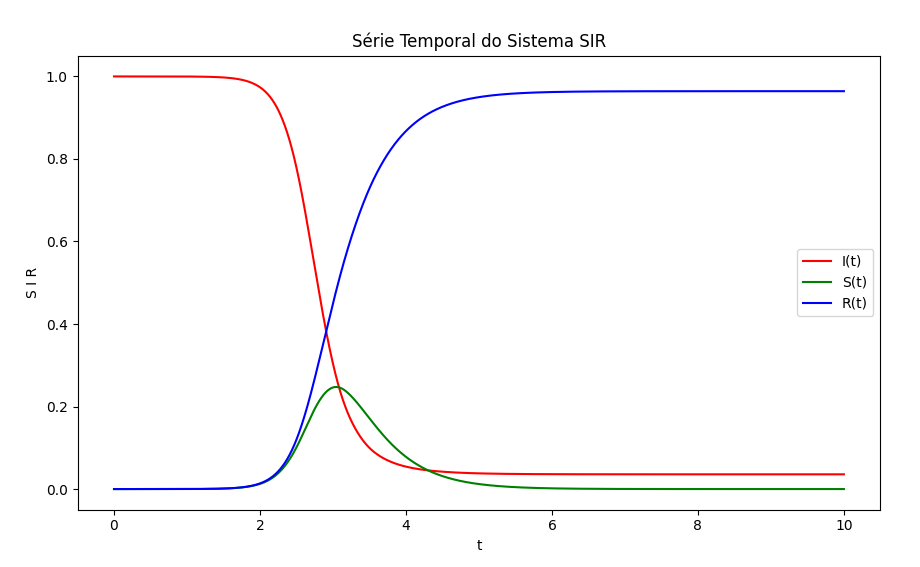
\includegraphics[width=0.8\textwidth]{images/SIR_rumos.png}
    %     \end{center}
    %     \caption{Gráfico SIR rumores}\label{fig:sir_rumors}
    % \end{figure}
    
    \begin{tikzpicture}[]
        % \node[anchor=south west] (image) at (0,0) {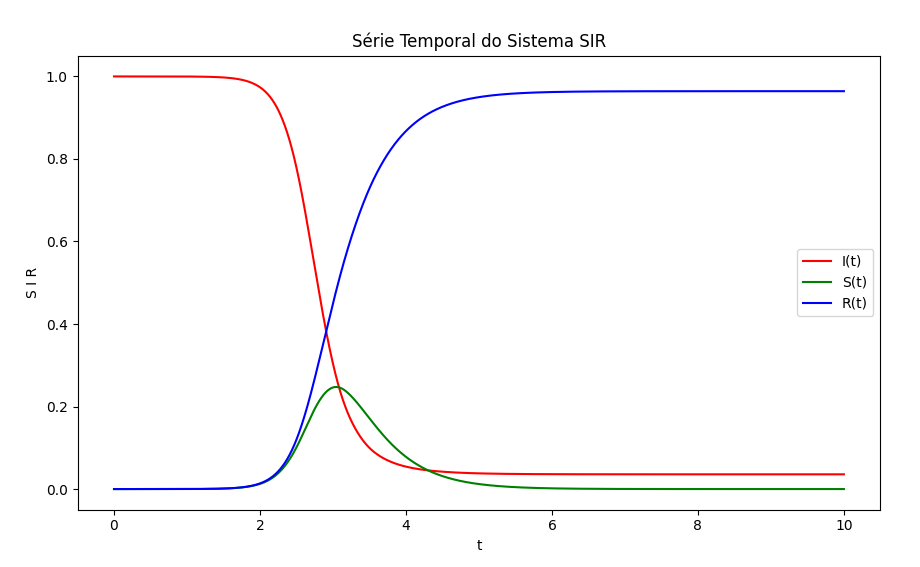
\includegraphics[width=9cm]{images/SIR_rumos.png}};
        %
        % % Define positions for nodes to the right of the image
        % \node[right=1cm of image.north east, anchor=north west] (node1) {$\bar{k} = 10$};
        % \node[below=0.5cm of node1, anchor=west] (node2) {$\lambda = 0.5$};
        % \node[below=0.5cm of node2, anchor=west] (node3) {$\gamma = 0.2$};
        % \node[below=0.5cm of node3, anchor=west] (node4) {$\eta, \delta = 0.2$};

        \node[anchor=south west, inner sep=0] (image) at (0,0) {\adjustbox{width=9cm}{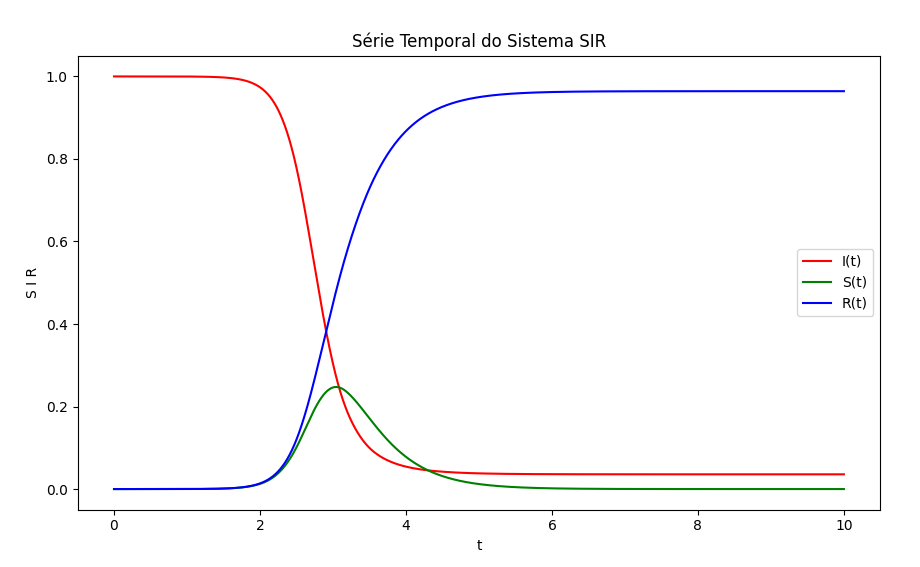
\includegraphics{images/SIR_rumos.png}}};

        \node at (10,5) {$\bullet  \bar{k} = 10$};   
        \node at (10, 4.5) {$\bullet \lambda = 0.5$}; 
        \node at (10, 4) {$\bullet \gamma = 0.1$};    
        \node at (10, 3.5) {$\bullet \eta = 0.2$}; 
        \node at (10, 3) {$\bullet \delta = 0.2$}; 

    \end{tikzpicture}

\end{frame}


%%%%%%%%%%%%%%%%%%%%%%%%%%%%%%%%%%%%%%%%%%%%%%%%%%%%%%%%%%%%%%%%%%%%%%%%%%%%%%%%%%%%%%%%%%%%%

\begin{frame}{Referências}


\begin{thebibliography}{2}



\beamertemplatearticlebibitems
\bibitem{Neves1976CharacterizationOJ}
K. W. Neves and A. Feldstein,
\newblock Characterization of jump discontinuities for state dependent delay differential equations.
\newblock \emph{Journal of Mathematical Analysis and Applications},
\oldstylenums{56}:689-707,
\oldstylenums{1976}.
\newblock \url{https://api.semanticscholar.org/CorpusID:121097839}.

 
\end{thebibliography}
\end{frame}


%%%%%%%%%%%%%%%%%%%%%%%%%%%%%%%%%%%%%%%%%%%%%%%%%%%%%%%%%%%%%%%%%%%%%%%%%%%%%%%%%%%%%%%%%%%%%%%%

\begin{frame}{Referências}


\begin{thebibliography}{2}


\beamertemplatearticlebibitems
\bibitem{NEVES1976689}
K. W. Neves and A. Feldstein,
\newblock Characterization of jump discontinuities for state dependent delay differential equations.
\newblock \emph{Journal of Mathematical Analysis and Applications},
\oldstylenums{56}(3):689-707,
\oldstylenums{1976}.
\newblock \url{https://doi.org/10.1016/0022-247X(76)90033-0}.

\beamertemplatearticlebibitems
\bibitem{NEVES1992385}
K. W. Neves and S. Thompson,
\newblock Software for the numerical solution of systems of functional differential equations with state-dependent delays.
\newblock \emph{Applied Numerical Mathematics},
\oldstylenums{9}(3):385-401,
\oldstylenums{1992}.
\newblock \url{https://doi.org/10.1016/0168-9274(92)90029-D}.
 


\beamertemplatebookbibitems
\bibitem{zennaro}
A. Bellen and M. Zennaro,
\newblock \emph{Numerical Methods for Delay Differential Equations}.
\newblock Oxford University Press,
\oldstylenums{2003}.
\newblock \url{https://doi.org/10.1093/acprof:oso/9780198506546.001.0001}.
 
\end{thebibliography}
\end{frame}


%%%%%%%%%%%%%%%%%%%%%%%%%%%%%%%%%%%%%%%%%%%%%%%%%%%%%%%%%%%%%%%%%%%%%%%%%%%%%%%%%%%%%%%%%%%%%%%%


\section{Referências}
\begin{frame}{Referências}


\begin{thebibliography}{3}

\beamertemplatearticlebibitems
\bibitem{PhysRevE.66.016128}
M. E. J. Newman,
\newblock Spread of epidemic disease on networks.
\newblock\emph{Phys. Rev. E},
\oldstylenums{66}(1):016128,
\oldstylenums{2002}.

\beamertemplatearticlebibitems
\bibitem{PhysRevE.64.026118}
M. E. J. Newman, S. H. Strogatz, and D. J. Watts,
\newblock Random graphs with arbitrary degree distributions and their applications.
\newblock\emph{Phys. Rev. E},
\oldstylenums{64}(2):026118,
\oldstylenums{2001}.


\beamertemplatebookbibitems
\bibitem{Author1990}M. E. J. Newman \newblock\emph{Networks}.\newblock
\textlatin{Oxford University Press, \oldstylenums{2018}}.

\end{thebibliography}
\end{frame}



%%%%%%%%%%%%%%%%%%%%%%%%%%%%%%%%%%%%%%%%%%%%%%%%%%%%%%%%%%%%%%%%%%%%%%%%%%%%%%%%%%%%%%%%%%%%%


\end{document}

